\documentclass[11pt]{article}

\usepackage[a4paper, margin=0.5cm, bmargin=1.2cm]{geometry}

\usepackage[utf8]{inputenc}
\usepackage[T1]{fontenc}

\pagenumbering{arabic}

\usepackage{mathtools}
\usepackage{amsmath}
%\usepackage{enumerate}
\usepackage[shortlabels]{enumitem}
\setlist[enumerate]{itemsep=2mm}


\usepackage{tikz}
\usetikzlibrary{calc,shapes.multipart,chains,arrows}
\usepackage{tikz-qtree}
\tikzset{every tree node/.style={minimum width=2em, minimum height=2em,draw},
         blank/.style={draw=none},
         edge from parent/.style=
         {draw,edge from parent path={(\tikzparentnode) -- (\tikzchildnode)}},
         level distance=1.5cm, sibling distance=0.5cm}

\usepackage{graphicx}
\usepackage[export]{adjustbox}
\usepackage{wrapfig}
\graphicspath{ {./images/} }

\usepackage{multicol}
\setlength{\columnsep}{0.5cm}
\usepackage{xcolor}

\definecolor{dkgreen}{rgb}{0,0.6,0}
\definecolor{gray}{rgb}{0.5,0.5,0.5}
\definecolor{mauve}{rgb}{0.58,0,0.82}
\definecolor{palegold}{rgb}{0.9, 0.7, 0.6}
\definecolor{darkslategrey}{RGB}{47,79,79}
\definecolor{intellijkeyword}{RGB}{204, 120, 50}
\definecolor{intellijstring}{RGB}{106, 135, 89}
\definecolor{intellijint}{RGB}{104, 151, 187}

\usepackage{hyperref}
\hypersetup{
	colorlinks=true,
	linkcolor=black,
	urlcolor=blue
}

\usepackage{listings}

\lstset{
    frame=tb,
    xleftmargin=5mm,
    language=Java,
    aboveskip=3mm,
    belowskip=3mm,
    showstringspaces=false,
    columns=flexible,
    basicstyle={\small\ttfamily},
    numbers=left,
    numberstyle=\tiny\color{red},
    keywordstyle=\color{intellijkeyword},
    commentstyle=\color{dkgreen},
    stringstyle=\color{intellijstring},
    breaklines=true,
    breakatwhitespace=true,
    tabsize=3,
    otherkeywords={;},
}


\usepackage[parfill]{parskip}

\usepackage{imakeidx}
\makeindex


\begin{document}

\tableofcontents
\newpage

\part{Kapittel 1: Grunnleggende begreper og teknikker}

\section{1.1 Algoritmer og effektvivitet}
    \subsection{1.1.3 Algoritmers effektivitet}
        Hva menes så med en arbeidsoperasjon? En arbeidsoperasjon er enten sammensatt (eng:
        compound) eller grunnleggende (eng: primitive). Den kalles grunnleggende hvis den ikke kan
        deles opp i enklere operasjoner. Det er ingen bestemt regel for dette, men en kunne for
        eksempel (på et mer overordnet nivå) kalle flg. operasjoner for grunnleggende: 
        \begin{enumerate}
            \item en tilordning - en variabel får en verdi
            \item en tabelloperasjon - en tabellverdi aksesseres
            \item sammenligning - to verdier sammenlignes
            \item en regneoperasjon - f.eks. en addisjon av to tall
        \end{enumerate}

        \subsubsection{Algoritmeeffektivitet - oppsummering}
            \begin{enumerate}
                \item En algoritme er en beskrivelse av de arbeidsoperasjonene som skal til for å løse en bestemt oppgave.
                \item Den har vanligvis en dominerende operasjon - f.eks. det å sammenligne.
                \item Vi kan telle opp antallet ganger den dominerende operasjonen utføres.
                \item Antallet kan ofte uttrykkes som en funksjon av oppgavens størrelse n. Denne funksjonen definerer algoritmens orden.
                \item Algoritmens orden er en målestokk for dens effektivitet.
                \item Jo mindre en algoritmes orden er, jo mer effektiv er den. F.eks. er lineær orden generelt mer effektivt enn kvadratisk orden. Tabell 1.8.2 viser de funksjonene som vi oftest kommer i kontakt med i algoritmeanalyse.
                \item Maks-metoden (Programkode 1.1.2) har lineær orden (orden n). Den er effektiv. Det er umulig å finne den største i en usortert tabell med færre enn n - 1 sammenligninger. Men koden kan optimaliseres noe (Avsnitt 1.1.4).
            \end{enumerate}

    \subsection{1.1.9 Det Harmoniske Tallet}
        Det Harmoniske Tallet ($H_n$) er gitt ved : \\
        $H_n = log(n) + 0.577$, der n er antall elementer i imput-arrayet. \\
        Dette gir gjennomsnittet av antall tall i arrayet som er mindre enn det minste tallet så langt.

    \subsection{1.1.12 Oppsummering}
        \begin{enumerate}
            \item En algoritme er en beskrivelse av de arbeidsoperasjonene som skal til for å løse en
                bestemt oppgave. Hvis det finnes flere algoritmer som løser den samme oppgaven, bør
                vi selvfølgelig velge den beste. Hvilken som er best er situasjonsbestemt. Eksempel:
                Vi skal sortere en samling verdier. Da er kanskje én algoritme best hvis det er mange
                verdier, mens en annen er kanskje best hvis det er få verdier. Slike spørsmål vil vi
                diskutere mange ganger i dette faget.
            \item Når vi lager programkode for en algoritme, skal vi normalt bruke standard kodeteknikk
                og sørge for at koden blir klar, lett forståelig og godt lesbar. Da vil moderne
                kompilatorer ofte være i stand til å optimalisere koden for oss. Men vi bør selvfølgelig
                unngå å lage unødvendig ineffektiv kode. Spesielt skal vi være oppmerksomme på
                operasjoner som utføres mange ganger, dvs. operasjoner som inngår i løkker. Der er
                det viktig å unngå unødvendig arbeid.
            \item Et stort programsystem vil inneholde mange algoritmer. En erfaring er at enkelte deler
                av programsystemet utføres oftere enn de øvrige. Det kan være så skjevt at 80 prosent
                programtiden foregår i 20 prosent av koden. Derfor bør man under programmeringen
                bruke anerkjente teknikker og sørge for god programstruktur. Hvis det så under
                testingen skulle vise seg at programmet har flaskehalser, så er det der en bør gå inn
                med lure teknikker for å øke effektiviteten.
        \end{enumerate}

\section{1.2 Den nest største verdien i en tabell}
    \subsection{1.2.1 Tabellintervaller}

        \subsubsection{Halvåpent Intervall}
            Parametrene fra og til er grensene for det halvåpne tabellintervallet
            a[fra:til$>$. Det består av elementene i a fra og med fra og til (men ikke med) til: \\
            a[fra:til$>$

        \subsubsection{Lukket Intervall}
            I noen situasjoner er det mest naturlig at en tabellmetode arbeider i et
            lukket tabellintervall. La v og h betegne intervallets venstre og høyre endepunkt. Et lukket
            tabellintervall betegnes med a[v:h] og består av elementene i a fra og med indeks v til og
            med indeks h. \\
            a[v:h]
        
    \subsection{1.2.6 Effektivitet - gjennomsnittlig og det verste tilfellet}
        Når det gjelder effektivitet skal vi skille mellom følgende tre tilfeller: 
        \begin{enumerate}
            \item Den gjennomsnittlige effektiviteten (eng: average case)
            \item Effektiviteten i det mest ugunstige eller verste tilfellet (eng: worst case)
            \item Effektiviteten i det beste tilfellet (eng: best case)
        \end{enumerate}

    
    \subsection{1.2.10 Generelle turneringer}
        Anta at det er n deltagere. I idrett og spill brukes såkalt «walk over». Det betyr at noen av
        deltagerne går rett til andre runde. Men fra og med andre runde må antallet være på formen $2*k$. 
        Dette får vi til ved å la turneringstreet inneholde nøyaktig $2n - 1$ noder. Treet tegnes slik:

        Sett opp én node øverst (nivå 0), så 2 noder på nivå 1, så 4 noder på nivå 2, osv. \\
        For hvert nytt nivå nedover tegner vi nodene én og én fra venstre mot høyre. \\
        I det øyeblikket vi til sammen har tegnet $2n - 1$ noder, stopper vi. \\
        Da behøver ikke det siste nivået i treet inneholde så mange noder som det er plass til. \\

        Et turneringstre for n deltagere vil ha $2n - 1$ noder, derav n bladnoder og $n - 1$ indre noder.
        De n deltagerne/tallene skal legges inn i bladnodene. Vi fyller ut bladnodene med tall fra
        venstre mot høyre, først de på nest nederste rad og deretter de på nederste rad.
    
\newpage

    \subsection{1.2.11 Perfekte, komplette og fulle trær}

        \paragraph{Definisjon 1.2.11 a)} Et binærtre kalles perfekt (eng: a perfect binary tree)
        hvis alle nivåene i treet inneholder så mange noder som det er plass til.

        \paragraph{Definisjon 1.2.11 b)} Et binærtre kalles komplett (eng: a complete binary
        tree) hvis hvert nivå, unntatt det siste (nederste) nivået, inneholder så mange
        noder som det er plass til. På siste nivå kan det være færre enn det er plass til,
        men det må ligge tett med noder fra venstre.

        \paragraph{Setning 1.2.11} Et komplett binærtre med n noder har høyde  $h =\lceil log2(n+1)\rceil – 1 = \lfloor log2(n)\rfloor$

        \paragraph{Definisjon 1.2.11 c)} Et binærtre kalles fullt (eng: a full binary tree) hvis hver
        node har enten to eller ingen barn.

        \paragraph{Definisjon 1.2.11 d)} Et binærtre kalles et maksimumstre (eng: a max tree)
        hvis hver node, bortsett fra rotnoden, har en verdi som er mindre enn eller lik
        verdien i nodens forelder

        \paragraph{Definisjon 1.2.11 e)} Et binærtre kalles en maksimumsheap (eng: a max
        heap) hvis det er et komplett maksimumstre.


\section{1.3 Ordnede tabeller}

    \subsection{1.3.1 Permutasjoner}

        \textbf{Leksikografisk Rekkefølge}\\
        \begin{multicols}{2}
            Hvis en permutasjon er gitt, hva blir da den neste leksikografisk sett? Vi ser først
            på noen enkle tilfeller og deretter på et som er mer generelt. Vi starter med flg. permutasjon
            av tallene fra 1 til 10:

            \columnbreak
            
            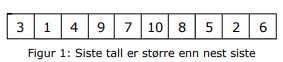
\includegraphics[center]{f-1.3.1-1.png}
            
        \end{multicols}

        \begin{multicols}{2}
            Hvis det siste tallet er større enn det nest siste (tallene 6 og 2 i Figur 1 over), får vi den
            neste i leksikografisk rekkefølge ved å bytte om de to. Med andre ord denne permutasjonen:
            
            \columnbreak
            
            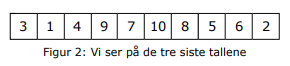
\includegraphics[center]{f-1.3.1-2.png}

        \end{multicols}

        \begin{multicols}{2}
            I Figur 2 er nå det siste tallet mindre enn det nest siste. Da nytter det ikke å bytte om dem.
            Vi må isteden trekke inn de tre siste tallene. De kan permuteres i leksikografisk rekkefølge på
            flg. seks måter: 2 5 6 , 2 6 5 , 5 2 6 , 5 6 2 , 6 2 5 og 6 5 2. Her ser vi at det er 6 2 5
            som kommer etter 5 6 2. Dermed blir dette neste permutasjon:

            \columnbreak

            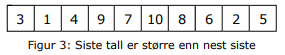
\includegraphics[center]{f-1.3.1-3.png}

        \end{multicols}

        \begin{multicols}{2}
            I Figur 3 har vi igjen den situasjonen at det siste tallet er større enn det nest siste. Dermed
            får vi neste permutasjon ved å bytte om de to:

            \columnbreak

            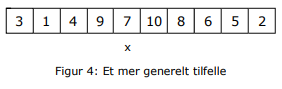
\includegraphics[center]{f-1.3.1-4.png}

        \end{multicols}

        Figur 4 viser et mer generelt tilfelle. Der er de fem siste tallene sortert avtagende. Generelt
        gjør vi slik for å finne den neste: Start bakerst og gå mot venstre så lenge som det er
        sortert. Dvs. vi skal stoppe på første tall som bryter sorteringen. I Figur 4 er det tallet 7
        (markert med en x). Neste skritt er: Bytt dette tallet med det minste av de til høyre
        som er større. I Figur 4 er tallet 8 det minste av de til høyre for 7 som er større enn 7. Snu
        så alle tallene til høyre for posisjon x. Dermed blir flg. permutasjon den som
        leksikografisk kommer etter den i Figur 4:

        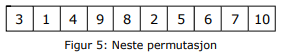
\includegraphics[center]{f-1.3.1-5.png}

    \subsection{1.3.3 Boblesortering}
        \subsubsection{Oppsummering - Boblesortering}
            \begin{enumerate}
                \item Navn: I en loddrett tabell, vil ombyttinger føre til at store verdier flytter seg oppover
                    og den største havner øverst. Navnet boble er hentet fra det som skjer når vannet i en
                    vannkjele koker. Da går det bobler oppover fra bunnen av kjelen.
                \item Effektivitet: Den forbedrede versjonen av boblesortering (Programkode 1.3.3 f ) er
                    (mhp. sammenligninger) av lineær orden (orden n) i det beste (en sortert tabell) og av
                    kvadratisk orden (orden n²) i gjennomsnitt og i det verste tilfellet.
                \item Ombyttinger: Antallet vil variere fra 0 (en sortert tabell) til $n(n - 1)/2$ (sortert motsatt
                    vei). I gjennomsnitt blir det $n(n - 1)/4$ ombyttinger.
                \item Konklusjon: Av de mest kjente sorteringsmetodene er boblesortering den som er
                    minst effektiv. Den brukes normalt ikke. I hvert fall ikke på store tabeller
            \end{enumerate}
        
    \subsection{1.3.4 Utvalgssortering}
        \subsubsection{Oppsummering - Utvalgssortering}
            \begin{enumerate}
                \item Navn: Algoritmen kalles utvalgssortering fordi det fortløpende velges ut en verdi
                    som så blir plassert på rett sortert plass. I den vanlige versjonen av utvalgssortering
                    blir fortløpende den minste blant de usorterte valgt ut og så plassert først blant dem.
                \item Effektivitet: Det trengs $n - 1$ sammenligninger for å finne den minste, så $n - 2$
                    stykker for å finne den nest minste (den minste av de øvrige), osv. Til sammen blir det
                    $n(n - 1)/2 = n^2/2 - n/2$ sammenligninger og det uansett fordelingen av verdiene. Det
                    betyr at algoritmen har kvadratisk orden i alle tilfeller (verst, gjennomsnittlig og best).
                \item Ombyttinger: Det gjøres én ombytting i hver iterasjon og dermed $n - 1$ til sammen.
                    Dette kan reduseres noe. Se Oppgave 11.
                \item Konklusjon: Utvalgssortering er som alle sorteringsalgoritmer av kvadratisk orden,
                    ikke egnet til å sortere store tabeller. Den er imidlertid bedre enn boblesortering. Se
                    Oppgave 4. I noen situasjoner kan det være ekstra kostbart å bytte om verdier (gjelder
                    ikke i Java). I slike tilfeller kan denne algoritmen brukes for tabeller av moderat
                    størrelse. Dette er den algoritmen som har færrest ombyttinger.
            \end{enumerate}

    \subsection{ 1.3.8 Ordnet innsetting, innsettings- og shellsortering}
        \subsubsection{Oppsummering - innsettingssortering}
            \begin{enumerate}
                \item Navn: Det kalles innsettingssortering fordi tabellen underveis er todelt. Venstre del
                    er sortert. Én og én verdi fra høyre del settes inn på rett sortert plass i venstre del. Ved
                    start består venstre del av det første elementet og høyre del av resten. Når algoritmen
                    slutter, består venstre del av hele tabellen (og høyre del er tom).

                \item Effektivitet: Det kan vises (se algoritmeanalyse) at det i gjennomsnitt (hvis alle
                    verdiene er forskjellige) utføres $n(n + 3)/4 - H_n$ sammenligninger. Det betyr at den er
                    av kvadratisk orden i gjennomsnitt. Hvis tabellen allerede er sortert, utføres det $n - 1$
                    sammenligninger. Dermed er den av lineær orden i det beste tilfellet.

                \item Ombyttinger: Det er ingen ombyttinger slik som innsettingssortering er kodet i
                    Programkode 1.3.8 c). Det er isteden forskyvninger (tilordninger) som er litt mindre
                    kostbare, og av dem er det i gjennomsnitt $n(n - 1)/4$ stykker.

                \item Konklusjon: Av de tre av kvadratisk orden som vi har sett på, er innsettingssortering
                    best. Vi skal se på algoritmer av orden n log(n) og de er langt bedre for store tabeller.
                    Men innsettingssortering er best hvis tabellen er liten eller stor, men delvis sortert. Det
                    er kvikksortering som er best av de avanserte. Den arbeider på intervaller og når
                    de har blitt små nok, er det der vanlig å skifte over til innsettingssortering.
            \end{enumerate}

        \subsubsection{Oppsummering - shellsortering}
            \begin{enumerate}
                \item Navn: Kalles shellsortering til ære for oppdageren Donald Shell. Den ble kjent i
                    1959 og vakte stor interesse siden man på den tiden ikke kjente til generelle metoder
                    med en (gjennomsnittlig) orden vesentlig bedre enn n².
                \item Effektivitet: Det er kjent at den er av kvadrastisk (n²) orden i det verste og av
                    orden n log(n) i det beste tilfellet. Men metoden er sterkt avhengig av sekvensen av
                    gap-verdier og det er ikke kjent hvilken orden den har i gjennomsnitt.
                \item Konklusjon: Metoden brukes ikke lenger i praksis siden det nå finnes bedre metoder -
                    f.eks. kvikksortering. Men den er interessant siden den på en systematisk måte utnytter
                    de beste sidene ved innsettingssortering.
            \end{enumerate}
    
    \subsection{1.3.9 Partisjonering og kvikksortering}
        Å partisjonere en tabell betyr å omorganisere og ordne den i deler etter bestemte kriterier. 

        \paragraph{Todelt partisjonering} Målet er å finne en algoritme som omorganiserer en tabell slik at
        alle verdier som er mindre enn en skilleverdi kommer først. Vi bruker Eksempel 1.3.9 b)
        som utgangspunkt. Tabellen kan, men behøver ikke, inneholde selve skilleverdien.

        \subsubsection{Oppsummering - Kvikksortering}
            \paragraph{Partisjonering}
            Å «dele» et sett med verdier slik at alt som er større
            enn eller lik en gitt skilleverdi ligger til høyre for verdien, og alt mindre ligger til
            venstre.

            \begin{enumerate}
                \item Navn: Kvikksortering (eng: quick sort)
                    ble «oppfunnet» allerede i 1959 av briten Tony Hoare
                    og er kjent som den beste (mest effektive) generelle sorteringsteknikken.
                    I java.util er det en optimalisert versjon (a dual-pivot quicksort) som brukes for standardtypene (byte, short, int, long, float, double, char).
                    Men for generiske typer brukes (i java.util) imidlertid flettesortering (eng: merge sort).
                \item Idé og effektivitet: Den kan ses på som en anvendelse av partisjonering, dvs. å dele en tabell (eller et tabellintervall) i to deler mhp. en skilleverdi (eng: pivot).
                    Et enkelt valg av skilleverdi kan være den første eller siste verdien. Men det vil føre til at den får orden n² hvis tabellen allerede er sortert. Da er det bedre å velge den midterste. Men i optimaliserte versjoner gjøres valget på en «lurere» måte.
                    Men uansett vil det være mulig (men ikke enkelt) å konstruere en tabell som gjør at den får orden n². Men i gjennomsnitt er den garantert av orden $n\cdot log(n)$. Se Oppgave 17. En mulig optimaliseringsteknikk er å skifte til innsettingssortering for små intervaller (lengde mindre enn 47 brukes i java.util). Den er en «på plass»-algoritme (eng: in place), dvs. at den ikke trenger noen hjelpetabell.
                \item Ulemper: Den optimaliserte versjonen vil, som nevnt over, kunne være av kvadratisk orden i (svært) spesielle tilfeller. Hvis en trenger en teknikk som alltid er $n\cdot log(n)$, må en velge noe annet - f.eks. heapsortering som alltid er av orden $n\cdot log(n)$, men som ikke er fullt så god som kvikksortering i gjennomsnitt. Et mulig valg er å kombinere de to slik det er gjort i introsort. En (liten) ulempe er at den ikke er stabil, dvs. like verdier får ikke nødvendigvis samme innbyrdes rekkefølge etter sorteringen som de hadde før.
                \item Konklusjon: Dette vil normalt være førstevalget når en trenger en sorteringsalgoritme.
            \end{enumerate}
\newpage

\section{1.4 Generiske algoritmer}
    \subsection{1.4.2 Sammenlignbarhet, grensesnitt og generiske metoder}
        I programmering brukes begrepet generisk både om metoder og klasser. Med tanke på
        avsnittet over burde en generisk metode virke eller kunne brukes for alle datatyper av samme
        «art». F.eks. kunne vi si at alle datatyper som er «sammenlignbare» (dvs. at instanser kan
        sammenlignes innbyrdes og ordnes i en bestemt rekkefølge) utgjør samme «art». 
    
    \subsection{1.4.3 Omslagsklasser}
        Det vil være upraktisk alltid å måtte kode en algoritme for alle aktuelle grunnleggende typer.
        Ta f.eks. en maks-metode. En helgardering tilsier at vi, i tillegg til den generiske versjonen i
        Programkode 1.4.2 b), også måtte lage versjoner for byte, short, int, long, char, float og
        double. Heldigvis har Java en teknikk som gjør det litt enklere for oss.

        Hver grunnleggende datatype kan «gjøres om» til en referansetype ved hjelp av en såkalt
        omslagsklasse (eng: wrapper class). For eksempel er klassen Integer en omslagsklasse for
        datatypen int. Klassen Integer har kun et heltall, dvs. en int, som instansvariabel. Navnet
        omslagsklasse kommer av at klassen fungerer som et omslag rundt datatypen.

        Java har en form for typekonvertering mellom int og Integer. Det kalles autoboksing (eng:
        autoboxing) og avboksing (eng: unboxing). En Integer kan ses på som et omslag (eller en
        boks) rundt et heltall. Bruker vi en int der syntaksen krever en Integer, vil kompilatoren
        automatisk legge et «omslag» rundt heltallet. Omvendt vil kompilatoren automatisk fjerne
        «omslaget» hvis vi bruker en Integer der syntaksen krever en int. 

    \subsection{1.4.9 Ordninger - Comparable versus Comparator}
        \paragraph{Comparable:} I overskriften på dette avsnittet står det Comparable versus Comparator. Gitt
        at vi skal lage en klasse der instanser vil kunne bli sammenlignet og ordnet. Skal vi da la den
        implementere Comparable (bli sammenlignbar) eller skal vi lage en Comparator som tar seg
        av ordningen? Her er det ingen fasit, men hvis det kan sies at instansene har en naturlig
        ordning, så er det vanlig å la klassen implementere Comparable. Tall har en naturlig ordning –
        de ordnes etter størrelse. Bokstaver og ord har også en naturlig ordning – de ordnes
        alfabetisk. Klokkeslett og datoer har naturlige ordninger – de ordnes i tidsrekkefølge.
        Personer kan sies å ha naturlig ordning – de ordnes normalt leksikografisk (etternavn og så
        fornavn). Det er ingen regel som forteller om en ordning er naturlig eller ikke. Det er ofte
        basert på skjønn. Men det er noen krav som må være oppfylt. Se nedenfor om compareTo().
        De forskjellige bibliotekene i Java 1.8 har hele 152 klasser som implementerer Comparable.
        Der inngår selvfølgelig klasser som Boolean, Byte, Short, Integer, Long, BigInteger, Float,
        Double, BigDecimal, Character, String, LocalTime, LocalDate og Calendar.

        \paragraph{Comparator:} Hvis instanser av en klasse som allerede er sammenlignbar (dvs. implementerer
        Comparable eller er en subtype til en slik en) skal ordnes på en spesiell måte, dvs. på en
        annen måte enn den «naturlige», må det lages en komparator for denne spesielle ordningen.
        Dette så vi eksempler på i Avsnitt 1.4.6 der det ble laget komparatorer for å ordne
        personer etter fornavn, studenter etter klasse og tegnstrenger etter lengde.
        Spesielt gjelder at hvis en klasse som ikke er sammenlignbar, skal ordnes på en en eller
        annen måte, så må vi lage en komparator for den ordningen. I følgende eksempel ser vi på
        punkter i et x, y - koordinatsystem. De har ingen naturlig ordning. Men det kan være måter å
        ordne dem på som er av interesse i spesielle situasjoner. F.eks. slik: Av to punkter er det
        «minst» som har minst x - koordinat. Hvis to punkter har like x - koordinater, er det «minst»
        som har minst y - koordinat, dvs. en leksikografisk ordning mhp. x - og y - koordinatene.

\newpage

        \subsubsection{Oppsumering}
            \paragraph{compareTo:} Hvis instanser av en klasse X har en «naturlig» ordning, så er det som nevnt
            over, vanlig å la X implementere Comparable<X>. Da må det være flg. sammenheng mellom
            compareTo og ordningen (x og y er to vilkårlige instanser av klassen X): 

            \begin{enumerate}
                \item x er «mindre enn» y hvis og bare hvis x.compareTo(y) < 0
                \item x er «mindre enn eller lik» y hvis og bare hvis x.compareTo(y) <= 0
                \item x er lik y hvis og bare hvis x.compareTo(y) = 0
                \item x.compareTo(y) < 0 hvis og bare hvis y.compareTo(x) > 0
            \end{enumerate}

            Det følger av punktene at x.compareTo(y) <= 0 hvis og bare hvis y.compareTo(x) >= 0. Det
            er vanligvis fordelaktig, men ikke et krav, at compareTo kodes slik at for alle x og y gjelder at
            x.compareTo(y) = -y.compareTo(x). I punktene inngår kun «mindre enn» og «mindre enn
            eller lik», men som vanlig defineres x «større enn» y som at y er «mindre enn» x. Tilsvarende
            er det for «større enn eller lik».

            Vi må også passe på metoden equals. Den må synkroniseres med compareTo siden begge
            kan brukes til å teste om to verdier er like. Kravet er at x.equals(y) = true hvis og bare
            hvis x.compareTo(y) = 0. Dette bør igjen synkroniseres med hashCode. Hvis equals sier at x
            og y er like, skal hashCode(x) = hashCode(y). Se også Avsnitt 1.4.12.

            \paragraph{compare:} Comparator har metoden compare, men når vi lager en komparator ved hjelp av
            et lambda-uttrykk, ser vi ikke den. Lambda-uttrykket er på formen (x,y) -> f(x,y) der f er
            en funksjon som returnerer et heltall. Komparatorordningen behøver ikke være en total
            ordning. Det holder at den er en total preordning. Flg. krav til sammenhengen mellom f
            og ordningen må være oppfylt:

            \begin{enumerate}
                \item x er «mindre enn» y hvis og bare hvis f(x,y) < 0
                \item x er «mindre enn eller lik» y hvis og bare hvis f(x,y) <= 0
                \item hvis x er lik y, så er f(x,y) = 0
                \item f(x,y) < 0 hvis og bare hvis f(y,x) > 0
            \end{enumerate}

            Det er vanligvis fordelaktig, men ikke et krav, at for alle x og y er f(x,y) = -f(y,x). Det er
            spesielt punkt 3 som skiller dette fra en total ordning. Vi kan ha at f(x,y) = 0 uten at x er
            lik y. Ta lamda-uttrykket i Programkode 1.4.6 i) som eksempel. Der er f gitt ved følgende
            uttrykk: f(x,y) = x.length() - y.length() der x og y er av typen String. Vi ser at f(x,y)
            = 0 så sant x og y er like lange. Men det behøver på ingen måte bety at x = y. Denne
            spesielle ordningen er en total preordning, men ikke en total ordning. I en slik ordning
            vil forskjellige elementer x og y med f(x,y) = 0 ikke ha noen spesiell innbyrdes ordning. 

\newpage
\section{1.5 Rekursjon}
    En rekursiv funksjon kaller seg selv.

    \subsection{1.5.3 Krav til rekursive metoder}

        \begin{enumerate}
            \item[Krav 1] Når metoden kalles seg selv én eller flere ganger må kallet (eller
                kallene) utføres på et tilfelle (eller en situasjon) som er enklere enn det tilfellet
                (den situasjonen) vi opprinnelig hadde. I tilegg må kallene være slik at ting ikke
                gjentas, dvs. at noe som allerede er løst ikke løses på nytt.

            \item[Krav 2] Metodekallene må utformes slik at det før eller senere oppstår et tilfelle
                (eller en situasjon) som kan behandles uten et nytt eller nye kall på metoden.
                Dette kalles et basistilfelle (eller en basissituasjon).
        \end{enumerate}

        Hvis en rekursiv metode oppfyller disse to kravene, skal den teoretisk sett virke. Men det vil
        være situasjoner der metoden likevel feiler. Hvis metoden f.eks. gjør svært mange rekursive
        kall før det oppstår et basistilfelle, vil rekursjonsdybden kunne bli så stor at det ikke lenger er
        plass til programstakken innenfor tilgjengelig minne. Da kastes en StackOverflowError. Vi
        må også her se på metodens orden, dvs. antallet operasjoner eller metodekall som utføres i
        forhold til oppgavens størrelse. Hvis metoden har en «dårlig» orden vil den være helt uegnet
        til å løse «store» problemer.


        \subsubsection{Fra LF} 
            \begin{enumerate}
                \item Ting kan ikke gjentas – ett kall til metoden med ett sett med argumenter kan kun
                forekomme en gang.
                \item All rekursjon må ende i et basistilfelle som er eksplisitt
                håndtert.
            \end{enumerate}

            Hvis en funksjon ikke oppfyller disse kravene risikerer man at den går i en evig løkke.
            Dette kan føre til StackOverFlow.

    \subsection{1.5.8 Flettesortering}
        Gitt to lister med sorterte tall,
        velg det minste fra de to listene til enhver tid. \\

        \begin{enumerate}
            \item Rekursivt del opp listen i to, til den ikke lenger kan bli delt opp.
            \item Slå sammen listen i sortert rekkefølge.
        \end{enumerate}


\section{1.6 Multidimensjonale tabeller og matriser}
    \textbf{[IKKE SKREVET]}

\section{1.8 Algoritmeanalyse}

    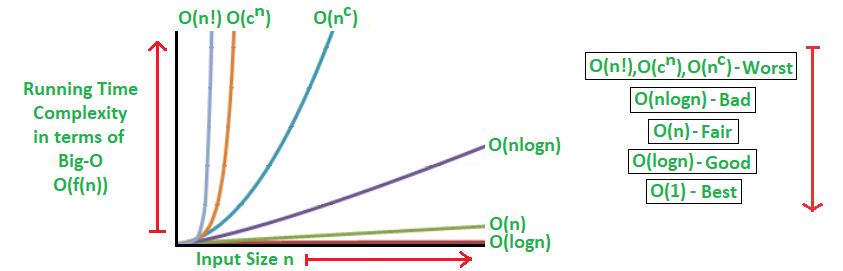
\includegraphics[center]{big_o.png}

\newpage

    \subsection{1.8.1 En algoritmes arbeidsmengde}
        \begin{enumerate}
            \item \textbf{Arbeidsoperasjoner} En algoritme er en beskrivelse av de arbeidsoperasjonene som skal
                til for å løse en bestemt oppgave.
            \item \textbf{Oppgave, algoritme og implementasjon} Våre oppgaver vil være slike som kan løses
                ved hjelp et program (eller en metode) skrevet i f.eks. Java. Vi skiller mellom selve
                oppgaven, en algoritme for å løse oppgaven og en implementasjon (kode) av algoritmen.
                Det er ofte flere måter å løse en oppgave, dvs. flere mulige algoritmer for samme oppgave
                og en bestemt algoritme kan ofte kodes på flere måter.
            \item \textbf{Dominerende operasjon}  Blant arbeidsoperasjonene er det vanligvis en som er viktigere,
                er mer sentral eller er mer kostbar og utføres oftere enn de andre. Det kalles den
                dominerende operasjonen. F.eks. er det å sammenligne to verdier en dominerende
                operasjon i vanlig sortering. I numeriske algoritmer (algoritmer med tallberegninger) kan
                f.eks. en multiplikasjon (eller kanskje en divisjon) være en dominerende operasjon.
            \item \textbf{Arbeidsmengde} I mange algoritmer er det mulig å telle opp antallet ganger den
                dominerende operasjonen utføres. Dette antallet utgjør algoritmens arbeidsmengde.
            \item \textbf{Orden} Arbeidsmengden kan ofte uttrykkes som en funksjon av oppgavens størrelse n.
                Denne funksjonen definerer algoritmens orden.
        \end{enumerate}

    \subsection{1.8.2 Den asymptotiske rangeringen av funksjoner}
        Tabell 1.8.2
        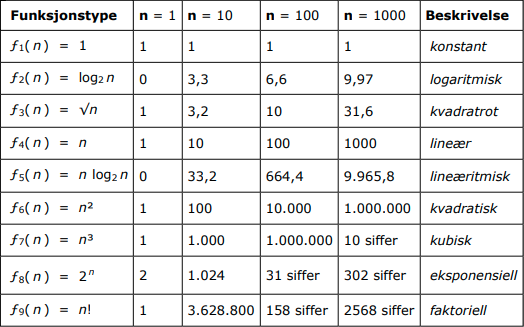
\includegraphics{Tabell-1.8.2.png}

        \paragraph{Dominerende Ledd}
        La funksjonen f( n ) være en lineærkombinasjon av flere
        ledd fra Tabell 1.8.2. Det av leddene i f( n ) som står lengst ned i Tabell 1.8.2
        (det største leddet), bestemmer den asymptotiske oppførselen til f( n ). Dette
        leddet kalles funksjonens dominerende ledd.

        \paragraph{Algoritmeorden}
        Anta at vi har en algoritme som løser en oppgave av
        størrelse n og at arbeidsmengden er gitt som en funksjon av n. Hvis g ( n ) er
        funksjonens dominerende ledd, sier vi at algoritmen er av orden g ( n ).

        \paragraph{Eksempel 1}
        Hvis arbeidsmengden til en algoritme er gitt ved $f( n ) = 2 n² + 3 n + log_2 n - 1$,
        så er algoritmen av orden n² eller av kvadratisk orden.
        \paragraph{Eksempel 2}
        La arbeidmengden til en algoritme være gitt ved $f( n ) = 0,2 \sqrt{n} + 10 log_2 n + 8$.
        Da er algoritmen av orden $\sqrt{n}$ eller av kvadratrotorden.

    \subsection{1.8.5 Notasjon med O, $\Omega$  og $\Theta$}
        \paragraph{O-notasjon, asymptotisk øvre grense}
        La f og g være to reelle funksjoner
        definert for reelle tall. Da sies f å være $O(g)$ (leses som O av g) hvis det finnes to
        faste tall (konstanter) $a$ og $n_0$ slik at $| f(n) | \leq a | g(n)|$ for alle $n \geq n_0$ .

        \paragraph{$\Omega$-notasjon, asymptotisk nedre grense}
        La f og g være to reelle funksjoner
        definert for reelle tall. Da sies f å være $\Omega(g)$ hvis det finnes en positiv konstant a
        og en konstant $n_0$ slik at $|f(n)| \geq a|g(n)|$ for alle $n \geq n_0$ .

        \paragraph{$\Theta$-notasjon, asymptotisk likhet}
        La f og g være to reelle funksjoner
        definert for reelle tall. Da sies f å være $\Theta(g)$ hvis det finnes positive konstanter
        a1 , a2 og en konstant $n_0$ slik at $a_1|g(n)| \leq |f(n)| \leq a_2|g(n)|$ for alle $n \leq n_0$ .

        \paragraph{Asymptotisk mindre enn}
        Vi sier at funksjonen f er asymptotisk mindre
        enn eller lik funksjonen g hvis f er O(g) og at f er asymptotisk mindre enn g
        hvis f er O(g) uten at de er asymptotisk like.

        \paragraph{En algoritmes orden}
        Anta at arbeidsmngden til en algoritme er gitt som
        funksjonen f(n). Hvis f er $\Theta(g)$, sier vi at algoritmen er av orden g.


        \subsubsection{Common Data Structure Operations}

            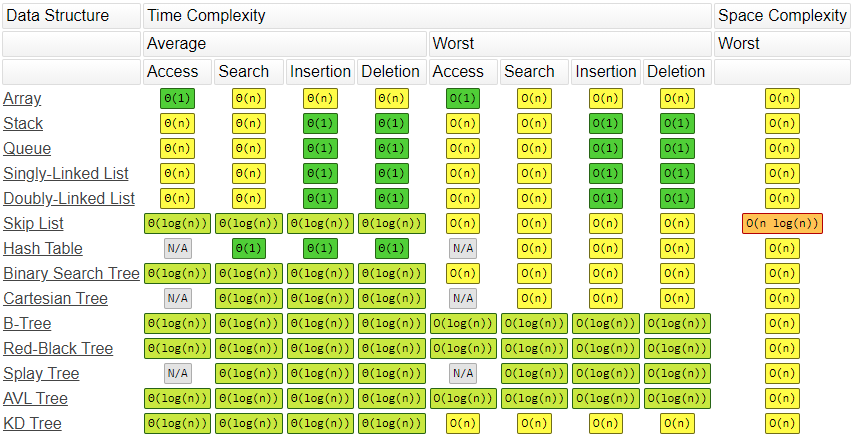
\includegraphics[scale=0.8]{common_ds_ops-new.png}

        \subsubsection{Array Sorting Algorithms}

            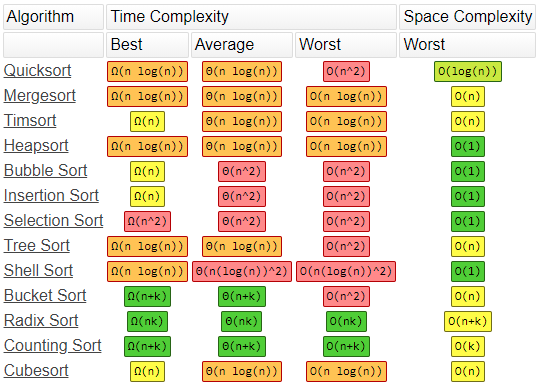
\includegraphics[center]{array_sorting_algs-new.png}

\newpage
\setcounter{part}{2}
\part{Kapittel 3: Lineære datastrukturer}
\section{3.1 En beholder}
    \subsection{3.1.1 En beholder}
        \subsubsection{Iterator}
            \begin{multicols}{2}
                En iterator kan ses på som en «innretning» som gjør det mulig å «bla» eller iterere
                gjennom en beholder. Å iterere betyr å utføre (gjenta) i rekkefølge. Itereringen skjer ved
                gjentatte kall på metoden next(). Da kommer hele innholdet fortløpende (en verdi om
                gangen) i en eller annen rekkefølge. Logisk sett burde det vært en metode first() som gir
                den første i rekkefølgen. Deretter skulle kall på next() gi den neste i forhold til det vi fikk
                sist. Men det er isteden laget slik, som kanskje er litt ulogisk, at første kall på next(), gir den
                første i rekkefølgen. Metoden hasNext() sjekker om det er flere igjen å se på i «beholderen».
    
                \columnbreak

                En iterator brukes normalt kun til å «bla»/iterere gjennom «beholderen». Men i mange
                tilfeller er det også mulig å fjerne objekter (ved hjelp av metoden remove) mens vi «blar».
                Metoden er satt opp som en standard metode (default) i grensesnittet. Det betyr at den
                formelt sett er kodet, men som «unsupported» (den kaster et unntak). Det betyr at hvis vi
                ønsker at den skal kunne brukes til å fjerne verdier, må vi selv kode den.
            \end{multicols}



\section{3.2 En tabellbasert liste}
    \subsection{3.2.1 Grensesnittet Liste}
        \subsubsection{Metodene i en liste skal oppfylle flg. krav: }
            \begin{enumerate}
                \item Metoden leggInn(T verdi) skal legge inn verdien verdi bakerst i listen.
                \item Metoden leggInn(int indeks, T verdi) har to argumenter. Den første bestemmer
                hvor verdi skal legges. Det betyr at de opprinnelige verdiene i listen fra og med
                posisjon indeks og utover vil få sine posisjoner økt med 1. Vi kan si at de forskyves
                mot høyre (eller nedover om vi vil) i listen. Hvis indeks er negativ eller er større enn
                antallet verdier, skal det kastes en IndexOutOfBoundsException. Det er imidlertid lovlig
                med indeks lik antallet verdier. Det betyr at den nye verdien skal legges bakerst.
                \item Metoden inneholder(T verdi) skal gi sann hvis den inneholder verdi og usann ellers.
                \item Metoden hent(int indeks) skal hente (uten å fjerne) verdien på indeks. Hvis den er
                negativ eller >= antallet i listen, skal det kastes en IndexOutOfBoundsException.
                \item Metoden indeksTil(T verdi) skal returner plassen/indeksen til første forekomst av
                verdi. Hvis den ikke finnes i listen returneres -1.
                \item Metoden oppdater(int indeks, T verdi) skal erstatte eksisterende verdi på indeks
                med verdien verdi. Den gamle verdien skal returneres. Hvis det er en ulovlig indeks
                (negativ eller >= antallet i listen) skal det kastes en IndexOutOfBoundsException.
                \item Metoden fjern(int indeks) skal fjerne (og returnere) verdien med denne indeksen.
                Antallet verdier blir dermed 1 mindre enn før, og alle verdiene som kommer etterpå får
                redusert sin indeks med 1. Hvis det er en ulovlig indeks (negativ eller >= antallet i
                listen) skal det kastes en IndexOutOfBoundsException.
                \item Metoden fjern(T verdi) skal fjerne første forekomst av verdi og returnere sann.
                Antallet verdier blir dermed 1 mindre enn før, og alle verdiene som kommer etterpå får
                redusert sin indeks med 1. Hvis verdi ikke er i listen, returneres usann.
                \item Metoden antall() skal returnere antallet verdier og dermed 0 hvis listen er tom.
                \item Metoden tom() skal returnere sann (true) hvis listen er tom og usann (false) ellers.
                \item Metoden nullstill() skal «tømme» listen, det vil si sørge for at det som eventuelt
                ligger igjen blir «resirkulert»og at listen deretter blir tom.
                \item Metoden iterator() skal returnere en iterator for listen.
                \item Default-metoden indeksKontroll(int, boolean) kan brukes av alle subklasser.
                Metoden leggInn(indeks,T) kan legge verdien bakerst, dvs. det er tillatt med indeks
                lik antall verdier i listen. Da brukes true som parameter i indeksKontroll(). Hvis det
                ikke er tillatt med indeks lik antall verdier, brukes false. 
            \end{enumerate}

\section{3.3 En lenket liste}

    \subsection{3.3.1 Lenket liste med noder}
        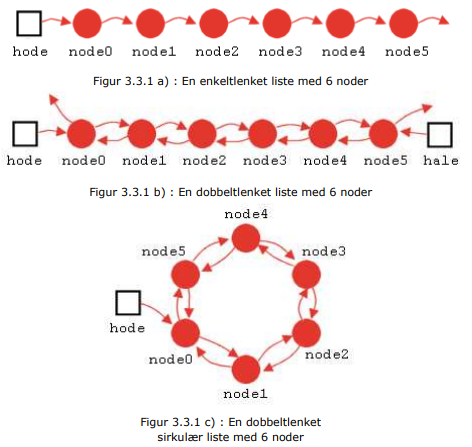
\includegraphics[center]{f-3.3.1abc.png}

        \textbf{Fjerning fra lenket list} \\
        Hvis indeks som skal fjernes er over halvparten av lengden på listen,
        starter vi bakerst. Hvis ikke starter vi forrest.

\newpage

    \subsection{3.3.5 Hvilken listeimplementasjon er «best»?}
        Vi kan gjøre flg. sammenligninger mellom de to listeimplementasjonene, dvs. TabellListe og
        EnkeltLenketListe:
        \begin{enumerate}
            \item TabellListe bruker tilsynelatende kun halvparten av plassen til EnkeltLenketListe.
            Det kommer av at hver node i EnkeltLenketListe har en nestereferanse i tillegg til en
            verdi. Men der brukes nøyaktig den plassen som trengs, mens den interne tabellen i
            TabellListe normalt lages en del større enn det som trengs i øyeblikket. Det betyr at
            de to likevel ikke adskiller seg så veldig mye med hensyn på plassbehov.
            \item Søking og oppdatering (metodene hent og oppdater) er av konstant orden i
            TabellListe og av orden n (der n er antallet verdier i listen) i EnkeltLenketListe.
            \item Det å legge en verdi bakerst i listen er av konstant orden for både TabellListe og for
            EnkeltLenketListe.
            \item Det å legge en verdi forrest i listen er av konstant orden i EnkeltLenketListe, men av
            orden n i TabellListe. Det kommer av at i TabellListe må alle verdiene flyttes før det
            kan legges noe forrest i tabellen.
            \item Det å legge en verdi på et vilkårlig sted i listen er av orden n for både TabellListe og
            for EnkeltLenketListe. I TabellListe er det å finne plassen av konstant orden, men
            det å flytte på verdier slik at plassen blir ledig, er av orden n. I EnkeltLenketListe er
            det å finne plassen av orden n, men det å flytte på verdier slik at plassen blir ledig, er
            av konstant orden.
            \item Metodene indeksTil, inneholder og fjern er av orden n både i TabellListe og i
            EnkeltLenketListe. I TabellListe er det å finne den som skal slettes av konstant
            orden, men det å «tette» igjen «hullet» i tabellen er av orden n. I EnkeltLenketListe
            er det å finne verdien av orden n, men det å ta vekk en node er av konstant orden.
        \end{enumerate}

\newpage
\part{Kapittel 4: Stakker og køer}

\section{4.1 En stakk (LIFO)}
    \paragraph{Definisjon}
        En stakk er en datastruktur der det alltid er den verdien som ble lagt
        på sist som står for tur til å bli tatt ut. Vi kan tenke på en stakk som en stabel av
        verdier der en ny verdi alltid legges øverst (på toppen) og der vi alltid (så sant
        stakken ikke er tom) tar den øverste hver gang en verdi skal tas ut.\\

        Et annet navn som også brukes på dette begrepet, er en "Sist-inn-først-ut"-kø. På engelsk
        heter det "Last-In-First-Out"-queue eller LIFO-queue.

    \subsection{4.1.2 En tabellbasert stakk}

        \begin{multicols}{2}
            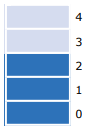
\includegraphics[center]{4.1.2-1.png}

                \columnbreak

            Det er ganske enkelt å implementere en stakk ved hjelp av en tabell. Da
            tenker vi oss at tabellen står på høykant - med indeks 0 nederst og med
            indeksene 1, 2, 3 osv. oppover. I figuren til venstre er det en tabell med plass
            til fem verdier. De tre nederste radene har mørk farge. Det skal indikere at der
            ligger det verdier. Med andre ord er antall verdier på «stakken» lik 3. De to
            øverste radene har lys farge. Det indikerer ledige plasser. Øverst på stakken er
            dermed den øverste av de «mørke». 
        \end{multicols}

    \subsection{4.1.3 Stakk ved hjelp av en pekerkjede}
        \begin{multicols}{2}

            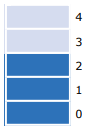
\includegraphics[center]{4.1.2-1.png}

            \columnbreak

            En stakk kan på en enkel måte implementeres ved hjelp av en
            enkeltlenket liste (pekerkjede.) Hvis listen tegnes vertikalt, vil den ligne
            på en stakk. Den første noden i listen blir da øverst av nodene (toppen
            av stakken) og den siste noden blir nederst (bunnen av stakken).

            I Figur 4.1.3 a) til venstre er en liste med fire noder tegnet vertikalt.
            Når et nytt objekt skal legges på toppen av stakken, representert ved
            hjelp av denne listen, må den tilhørende noden legges inn først, dvs.
            som en ny node 0. Metoden leggInn vil få konstant orden siden arbeidet
            med å legge inn noe først i en liste er uavhengig av antallet i listen.

            Metoden taUt (og kikk) vil også få konstant orden siden det å fjerne den
            første noden (node 0) i en liste har konstant orden.

            I en enkeltlenket liste er det vanlig å ha en halepeker (peker til den
            siste noden). Da vil det å legge inn et objekt bakerst i listen kunne
            gjøres effektivt. Men det er det ikke behov for her. 
            
        \end{multicols}

\newpage
\section{4.2 En kø (FIFO)}
    \subsection{4.2.1 Grensesnittet Kø}
        \paragraph{Definisjon}
        En kø er en datastruktur der verdier legges inn bakerst og tas ut
        forrest. Med andre ord er den verdien som ble lagt inn først (den som har ventet
        lengst) som tas ut først.\\

        Et annet navn som også brukes på dette begrepet, er en "Først-inn-først-ut"-kø. På engelsk
        heter det "First-In-First-Out"-queue eller FIFO-queue.

    \subsection{4.2.2 En sirkulær kø}
        \paragraph{Oppsummering}
        \begin{enumerate}
            \item  Køen skal ligge i en "sirkulær" tabell a.
            \item En variabel fra skal markere den første i køen (starten på køen). Den settes til 0 hvis
                en økning har gjort at den har blitt lik a.length.
            \item En variabel til skal markere første ledige, dvs. én posisjon forbi den siste i køen. Den
                settes til 0 hvis en økning har gjort at den har blitt lik a.length.
            \item Tabellen må utvides med en gang hvis den har blitt full etter en innlegging.
            \item  Hvis punktene foran er oppfylt, vil køen være tom hvis og bare hvis fra og til er like.
        \end{enumerate}

        \paragraph{Effektivitet}
        I starten av avsnittet ble det sagt at vanlig køkultur tilsier at når den første
        går ut av køen, beveger alle de andre seg et skritt fremover. Denne i og for seg fornuftige
        idéen er det umulig å implementere effektivt. Vi fant at en sirkelformet kø er et smart
        alternativ. Da beveger køen seg rundt i en sirkel, mens hver enkelt køståer er i ro inntil hun
        forlater køen. Dette fører til at både innlegging, kikking og uttak får konstant orden. Bedre
        enn det kan det ikke gjøres. Noen metoder kan kanskje optimaliseres litt. Se Avsnitt 4.2.3.

    \subsection{4.2.4 En lenket kø}
        Det er mulig å implementere en kø ved hjelp av en enkeltlenket liste med hode og hale. Køen
        starter ved hodet og slutter ved halen. Det å legge inn en verdi på slutten vil være av
        konstant orden. Det samme for det å ta ut (eller kikke på) den første i køen. Med andre ord
        vil både leggInn(), kikk() og taUt() da bli effektive operasjoner.

        \paragraph{Oppsummering}
        \begin{enumerate}
            \item Køen skal organiseres som en sirkelformet pekerkjede med en fast startstørrelse.
            \item En peker fra skal gå til den første i køen.
            \item En peker til skal gå til den første ledige noden, dvs. én forbi den siste i køen.
            \item Hvis til == fra, er køen tom.
            \item Køen skal aldri være full. Ved en innlegging skal det alltid være en ledig node. Hvis det
            er kun én, utvides pekerekjeden med en ekstra node mellom til og fra.
            \item En antall-variabel holder orden på antallet verdier i køen.
        \end{enumerate}

\newpage
\section{4.3 En toveiskø (Deque)}
    \subsection{4.3.1 Grensesnittet Toveiskø}
        
        \paragraph{Definisjon}
        En stakk kan godt ses på som en kø der vi kun legger inn i og tar ut fra den ene enden av
        køen. I en vanlig kø derimot legger vi inn i den ene enden (bakerst) og tar ut fra den andre
        enden (forrest). Begge disse ideene kan forenes i én type kø, dvs. en kø der vi både kan
        legge inn i begge ender og ta ut fra begge ender. En slik kø skal vi her kalle en toveiskø. Det
        engelsk navnet for dette er deque og ordet er en forkortelse for double ended queue.

        \paragraph{Som Stakk}
        En toveiskø kan fungere som en stakk ved at metodene leggInnFørst, kikkFørst og
        taUtFørst brukes som push, peek og pop. Eller en kan bruke leggInnSist, kikkSist og taUtSist.
        Begge ender av toveiskøen skal fungere på samme måte.
            
        \paragraph{Som Kø}
        En toveiskø kan fungere som en vanlig kø ved at leggInnSist, kikkFørst og taUtFørst
        brukes som push, peek og pop. Eller eventuelt leggInnFørst, kikkSist og taUtSist.

    \subsection{4.3.2 Lenket toveiskø}
        En enkel måte å konstruere en toveiskø på er å bruke en toveis pekerkjede (dobbeltlenket
        liste) som intern datastruktur. Der brukes vanligvis hode og hale som navn på starten og
        slutten av listen. Her velger vi imidletid start og slutt siden det passer bedre i en toveiskø. 

    \subsection{4.3.3 Sirkulær toveiskø}
        En sirkulær toveiskø bruker samme idé som i den sirkulære køen i Avsnitt 4.2.2. Vi kan derfor
        starte med klassen TabellKø og så bytte ut navnet TabellKø med navnet TabellToveiskø
        alle aktuelle steder. Videre bytter vi ut navnene på metodene leggInn(), kikk() og tauT()
        til henholdsvis leggInnSist(), kikkFørst() og taUtFørst(). Metodene utvidTabell(),
        antall(), tom(), nullstill() og toString() kan brukes som de er.


\section{4.4 En prioritetskø}
    \subsection{4.4.1 Grensesnittet PrioritetsKø}

        \paragraph{Definisjon}
        En prioritetskø (engelsk: priority queue) er en kø der de som "står" i
        køen har en prioritet. Da er regelen at den som har "best" eller
        "høyest" prioritet står først for tur til å bli tatt ut. En konsekvens er at
        den som har "lav" prioritet kan oppleve å måtte vente lenge

    \subsection{4.4.2 En prioritetskø ved hjelp av en usortert tabell}
        Prioritetskøen kan ha en usortert dynamisk tabell som intern datastruktur. Vi bestemmer at
        det objektet som en komparator sier er minst, er det som har best/høyest prioritet.

        Når tabellen er usortert kan nye verdier legges bakerst. Innlegging får derfor
        konstant orden. 

        Men det å finne den som har best/høyest prioritet, dvs. det minste tallet, krever at vi må lete
        gjennom hele tabellen. Til det kan vi f.eks. bruke en metode som finner posisjonen til den
        minste verdien i et tabellintervall. Det betyr at det å ta ut en verdi får lineær orden. Når vi tar ut et element,
        flytter vi det bakerste elementet til den plassen.

    \subsection{4.4.3 En prioritetskø ved hjelp av en sortert tabell}
        Elementet med høyest prioritet ligger bakerst. Å ta ut vil da ha konstant orden.

        Å legge inn vil ha lineær order O(n), siden riktig plass må finnes, og elementene bak må flyttes.

\newpage
\part{Kapittel 5: Binære trær}

\section{5.1 Binære trær}
    \subsection{5.1.1 Binære trærs egenskaper}
        \paragraph{Definisjon}
        Et binærtre består av en samling noder (eng: node/nodes) (muligens en tom
        samling) og en samling kanter (eng: edge/edges) som forbinder par av noder:
        \begin{enumerate}
            \item Hvis treet ikke er tomt, har det en rotnode. Kalles også treets rot (eng: root).
            \item Til enhver node Y, unntatt rotnoden, hører det nøyaktig én node X som vi kaller dens
                foreldernode eller bare forelder (eng: parent). Det går en kant mellom noden Y og dens
                forelder X. Omvendt sier vi at Y er et barn (eng: children) til X. En node kan ha to, ett
                eller ingen barn. Det er kun mellom nodepar av typen barn/forelder det går kanter.
            \item Hvis en node har to barn er det ene venstre barn og det andre høyre barn. Hvis noden
                har bare ett barn defineres det enten som venstre barn eller som høyre barn
        \end{enumerate}

        \subsubsection{Begrep}
            \paragraph{Nivå}
            Nivå (eng: level) brukes vanligvis i forbindelse med høyder og høydeforskjell. Havnivå og
            nivåkurver er kjente uttrykk. Her skal vi bruke begrepet på en tilsvarende måte. Rotnoden er
            på nivå $\Theta$. Vi assosierer vanligvis en rot med noe som er nede i bakken og dermed er det
            rimelig å si at en rot befinner seg på $\Theta$-nivået. (En bør være klar over at i enkelte
            fremstillinger sies rotnoden å være på nivå 1.) Barna til rotnoden er på nivå 1, barnebarna på
            nivå 2, osv. Det er vanlig å tegne alle nodene som hører til samme nivå på en og samme
            (vannrette) rad. I Figur 5.1.1 a) tilhører f.eks. nodene D, E, F og G samme nivå, dvs. nivå 2.

            Begrepet generasjon henter vi fra slektstrær. Der kalles gjerne rotnoden for stamforelder
            (stammor eller stamfar) og nivåene svarer til generasjoner. Forskjellen er at stamforelder
            vanligvis kalles 1. generasjon. Dermed vil generasjon k være det samme som nivå k - 1.

            Hvis alle nivåene i treet har så mange noder som det er plass til, sier vi at treet er perfekt
            (eng: a perfect binary tree). I et binærtre er det plass til 1 node på nivå $\Theta$, 2 noder på nivå 1,
            4 på nivå 2, 8 på nivå 3, osv. Generelt er det plass til 2k
            noder på nivå k.

            \paragraph{Slektskap}
            Det er ikke bare begrepet generasjon vi låner fra slektstreet. Vi bruker også
            begreper som barn og forelder, barnebarn og besteforelder, oldebarn og oldeforelder,
            etterkommer (eng: descendant, successor) og forgjenger (eng: ancestor, predecessor). Det
            burde være innlysende hva disse begrepene står for i et binærtre. To noder kalles søsken
            (eng: sibling) hvis de har samme forelder. En node (forskjellig fra rotnoden) kalles enebarn
            hvis den ikke har søsken. En node kalles barnløs hvis den ikke har barn

            \paragraph{Subtrær}
            Enhver node kan ses på som rotnode i sitt eget tre, dvs. det treet som består av
            noden og alle dens etterkommere (barn, barnebarn, osv). En node har alltid to subtrær - et
            venstre subtre og et høyre subtre - der ett eller begge kan være tomme. Venstre subtre til
            en node er (hvis det ikke er tomt) det treet som har venstre barn som sin rotnode. Det blir
            tilsvarende for høyre subtre.

            På Figur 5.1.1 a) består det venstre subtreet til rotnoden A av nodene B, D, E, H, I, J, K, O, P,
            Q, R og S. Det høyre subtreet består av resten, dvs. C, F, G, L, M, N, T, U og V. Disse to
            subtrærne har igjen hver sin rotnode - B for det venstre og C
            for det høyre subtreet. Noden B har også to subtrær. Nodene
            D, H, I, O, P og Q utgjør det venstre og E, J, K, R og S det
            høyre. Noden G for eksempel, har også to subtrær, men det
            høyre er tomt. Det venstre subtreet til G består av N og V.

            \paragraph{Bladnoder og indre noder}
            Nodene kan deles opp i to typer
            - bladnoder og indre noder (eng: leaf node, inner node). En
            bladnode (eller et blad) er en node som ikke har barn, eller
            som har to tomme subtrær om en vil. Alle andre noder er
            indre noder. Det betyr at en indre node har ett eller to barn.
            I Figur 5.1.1 a) ser vi fort at nodene O, P, Q, R, S, L, T, U og
            V er bladnoder, og dermed at resten er indre noder.

            \paragraph{En vei}
            Vi kan orientere alle kantene i treet ved å si at en
            kants retning er fra forelder til barn, dvs. nedover. Vi sier at det går en vei (eng: path)
            mellom to noder X og Y hvis det er mulig å komme fra X til Y ved å følge kanter. Spesielt får
            vi at Y er en etterkommer av X hvis det går en vei fra X til Y, eller omvendt at X er en
            forgjenger til Y. Veilengden er antallet kanter på veien. I Figur 5.1.1 a) går det f.eks. en vei
            med lengde 4 fra noden A til noden V. Men det går f.eks. ingen vei fra noden L til noden V.

            \paragraph{Avstand}
            Hvis det går en vei fra noden X til noden Y (eller fra Y til X) sier vi at avstanden
            mellom dem er lik veilengden. Hvis det ikke går en vei mellom dem, må de ha en nærmeste
            felles forgjenger Z. Da sier vi at avstanden mellom X og Y er lik avstanden mellom Z og X
            pluss avstanden mellom Z og Y. I Figur 5.1.1 a) er C nærmeste forgjenger til L og V og
            avstanden mellom dem blir dermed 2 + 3 = 5.

            \paragraph{Høyden}
            Høyden til et binærtre er lengden på den lengste veien i treet. Treet i Figur 5.1.1 a) har
            dermed høyde 4. Den lengste veien må nødvendigvis starte i rotnoden A, og vi ser at ingen
            vei er lengre enn 4. En annen måte å si det på er at høyden er det samme som det største
            nivået i treet. Treet i Figur 5.1.1 a) har 4 som største nivå - altså er høyden 4. Et binærtre
            med bare én node har høyde $\Theta$ og spesielt skal vi si at et tomt tre har høyde -1.
            Høyden til en node X er høyden til det subtreet som har X som rotnode. Rotnodens høyde blir
            dermed det samme som høyden til hele treet.

            \paragraph{Dybden}
            Dybden til en node X er avstanden mellom rotnoden og noden X. Dermed kan vi si at høyden
            til et binærtre er dybden til den "dypeste" noden. I treet i Figur 5.1.1 a) er det mange noder
            som er "dypest". Det er alle nodene på den nederste nivået.

            \paragraph{Retninger}
            Vi tegner som sagt et binærtre opp-ned. Dermed vil oppover og nedover bli det
            omvendte av det normale med tanke på et botanisk tre. Nedover betyr nå i retning vekk fra
            roten. Tilsvarende blir oppover retning mot roten. Et uttrykk som "langt nede i treet" vil nå
            bety langt fra roten. Bunnen av et tre betyr så langt ned en kan komme. I Figur 5.1.1 a) går
            vi nedover når vi starter i rotnoden A og f.eks. går mot noden S.

            \paragraph{En gren}
            En gren i treet består av alle nodene fra rotnoden og ned til en bladnode. Det betyr at det er
            like mange grener i treet som det er bladnoder. I treet i Figur 5.1.1 a) er det 9 bladnoder og
            dermed 9 grener. Venstre gren er den som ender i den bladnoden som ligger lengst til
            venstre og høyre gren den som ender i den bladnoden som ligger lengst til høyre. I treet i
            Figur 5.1.1 a) blir det grenene (venstre) A, B, D, H, O og (høyre) A, C, G, N, V. (En node
            ligger til venstre for en annen node hvis den første kommer foran den andre i inorden. Se
            definisjonen av inorden). Høyden i treet blir det samme som lengden på lengste gren.

\newpage

    \subsection{5.1.2 Antallet forskjellige trær}
    To trær på samme form er \textbf{isomorfe}.

        \paragraph{Formel for å regne ut}

        \begin{multicols}{2}
            \begin{equation}
                C(n) = \frac{1}{n+1}\binom{2n}{n}
            \end{equation}
            
            \columnbreak

            Tallene dette gir kalles \textbf{Catalan-tallene}.\\
            De 10 første, fra C(0): \\
            1 1 2 5 14 42 132 429 1430 4862

        \end{multicols}


    \subsection{5.1.3 Nodenes posisjoner}
    Vi kan bruke flg. regel for å bestemme nodeposisjoner:\\
    Rotnoden har posisjon 1.\\
    Deretter brukes "barnereglen": \\
    Barna til en node med posisjon k har henholdsvis 2 k
    (venstre) og 2 k + 1 (høyre) som posisjonstall.

    \subsection{5.1.4 Nodeposisjoner og binære tall}
        \begin{enumerate}
            \item Hver node i et binærtre har en entydig posisjon (eller et posisjonstall) og det er nodens
                plassering i treet som bestemmer dette tallet.
            \item Rotnoden har alltid posisjon 1.
            \item Hvis k, k > 1, er posisjonen til en node, så er $\lfloor k/2 \rfloor$ posisjonen til nodens forelder.
            \item Hvis en node med posisjon k har et venstre barn, så er ventrebarnets posisjon lik 2k.
            \item Hvis en node med posisjon k har et høyre barn, så er høyrebarnets posisjon lik 2k + 1.
            \item Hvis k, k > 1, er en posisjon i binærtreet, så gir de binære sifrene til k oss veien fra
                rotnoden ned til denne posisjonen. Vi hopper over det ledende 1-tallet. Deretter går vi
                til venstre når det er 0 og til høyre når det er 1.
            \item Høyden i et tre er én mindre enn antallet binære siffer i treets største posisjonstall.
        \end{enumerate}

    \subsection{5.1.6 Traverseringer - nivåorden}
        Nodene besøkes nivå-for-nivå, fra venstre til høyre.

    \subsection{5.1.7 Preorden, inorden og postorden}

    \begin{multicols}{2}
        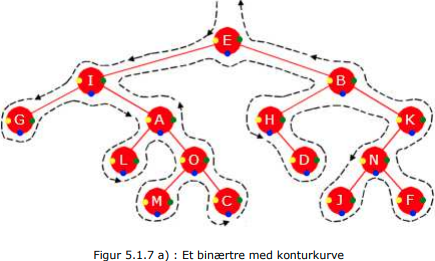
\includegraphics[scale=0.8]{figur.5.1.7a.png}

        \columnbreak

        Hvis vi starter ved rotnoden, følger konturkurven og skriver ut nodeverdiene ved passering av
        en farget "prikk", får vi flg. tre tilfeller: \\

        \begin{enumerate}
            \item Skriver vi ut nodeverdien når den gule "prikken" passeres, får vi verdiene i preorden.
                For treet i Figur 5.1.7 a) blir det E, I, G, A, L, O, M, C, B, H, D, K, N, J, F. Rotnoden
                kommer alltid først i preorden!
            \item  Skriver vi ut nodeverdien når den blå "prikken" passeres, får vi verdiene i inorden og
                dermed G, I, L, A, M, O, C, E, H, D, B, J, N, F, K for treet i Figur 5.1.7 a). Noden
                nederst til venstre kommer alltid først i inorden!
            \item  Skriver vi ut nodeverdien når den grønne "prikken" passeres, får vi dem i postorden.
                Det blir da G, L, M, C, O, A, I, D, H, J, F, N, K, B, E. Rotnoden kommer alltid sist i
                postorden!
        \end{enumerate}
        
    \end{multicols}




        \paragraph{Preorden - definisjon}
        Det er lettest å definere denne traverseringsrekkefølgen rekursivt: \\
        \begin{enumerate}
            \item Vi starter i rotnoden.
            \item Videre gjelder for alle noder at først "besøker" vi noden, så dens venstre barn hvis den
                har et venstre barn og så dens høyre barn hvis den har et høyre barn.
        \end{enumerate}
        \paragraph{Inorden - definisjon}
        Dette definerer vi også rekursivt:\\
        \begin{enumerate}
            \item Vi starter i rotnoden.
            \item Videre gjelder for alle noder at først "besøker" vi nodens venstre barn hvis den har et
                venstre barn, så noden og så dens høyre barn hvis den har et høyre barn.
        \end{enumerate}
        \paragraph{Postorden - definsjon}
        En rekursiv definisjon: \\
        \begin{enumerate}
            \item Vi starter i rotnoden.
            \item Videre gjelder for alle noder at først "besøker" vi nodens venstre barn hvis den har et
                venstre barn, så dens høyre barn hvis den har et høyre barn og så "besøker" vi noden
        \end{enumerate}

        \subsubsection{Neste Node}
            \paragraph{Preorden}
            \begin{enumerate}
                \item Hvis p har et venstre barn, så er det barnet den neste.
                \item Hvis p ikke har et venstre barn, men et høyre barn, så er det barnet den neste.
                \item Hvis p ikke har barn, dvs. p er en bladnode, så må vi først til den nærmeste (oppover
                    mot roten) noden q som har et høyre barn og som har p i sitt venstre subtre. Den neste
                    til p er da det høyre barnet til q.
                \item Hvis det ikke finnes noen slik q, er p den siste i preorden.
            \end{enumerate}

            \paragraph{Inorden}
            \begin{enumerate}
                \item Hvis p har et ikke-tomt høyre subtre, så er den neste den noden som kommer først i
                    inorden i det subtreet.
                \item Hvis p har et tomt høyre subtre, er den neste den nærmeste noden oppover mot roten
                    som har p i sitt venstre subtre.
                \item Hvis det ikke finnes noen slik node, er p den siste i inorden.
            \end{enumerate}

            \paragraph{Postorden}
            \begin{enumerate}
                \item Hvis p ikke har en forelder ( p er rotnoden), så er p den siste i postorden.
                \item Hvis p er høyre barn til sin forelder f, er forelderen f den neste.
                \item Hvis p er venstre barn til sin forelder f, gjelder:
                    \begin{enumerate}
                        \item Hvis p er enebarn (f.høyre er null), er forelderen f den neste.
                        \item Hvis p ikke er enebarn (dvs. f.høyre er ikke null), så er den neste den noden
                                som kommer først i postorden i subtreet med f.høyre som rot.
                    \end{enumerate}
            \end{enumerate}

\newpage
\section{5.2 Binære søketrær}
    \subsection{5.2.1 Hva er et binært søketre?}
        Navnet binært søketre (eng: binary search tree) indikerer at det er et binærtre som er
        tilrettelagt for søking. I Delkapittel 1.3 så vi på ordnede tabeller og binærsøk. Binærsøk er
        effektiv siden den er av logaritmisk orden. Det er imidlertid kostbart å vedlikeholde en ordnet
        tabell. Innlegging på rett sortert plass er av orden n. Også fjerning er av orden n siden
        "hullet" må tettes igjen. Et binært søketre er en datastruktur der søkingen i gjennomsnitt er
        omtrent like effektiv som binærsøk. I tillegg er også innlegging og fjerning i gjennomsnitt av
        logaritmisk orden. Prisen er imidlertid at vi bruker mer plass enn det en tabell trenger.


        \textbf{Definisjon}\\
        For at et binærtre skal kunne være et søketre, må treets verdier oppfylle flg. krav: 
        For hver node p gjelder:
            \begin{enumerate}
                \item Hvis p har et ikke-tomt venstre
                    subtre, er alle verdiene der mindre enn verdien i p.
                \item Hvis p har et ikke-tomt
                    høyre subtre, er alle verdiene der større enn eller lik verdien i p.
            \end{enumerate}
        Et tomt tre og et tre med kun én node er per definisjon et binært søketre.

        OBS: Definisjonen gir at verdiene i et binært søketre er sortert (stigende) i inorden. 

    \subsection{5.2.4 Gjennomsnittlig nodedybde}
        Det finnes en formel (den utledes i Avsnitt 5.2.15 ) for den gjennomsnittlige nodedybden Dn
        for binære søketrær med n noder. Den ser slik ut: 
            \[
                D_n = 2(1+\frac{1}{n}H_n-4)
            \]

        Hn er det n-te harmoniske tallet, dvs. summen av de inverse heltallene fra 1 til n. Hvis n er
        stor, vil 1/n ha liten effekt. Videre vil (se Avsnitt 1.1.6 ) Hn være tilnærmet lik log(n) + 0,577
        der log er den naturlige logaritmen (grunntall e). Formelen log(n) = log(2) · log2(n) der log(2)
        = 0,693, gjør om til grunntall 2. Det gir flg. formel for gjennomsnittlig nodedybde:
            \[
                D_n = 2H-4 \approx 1.386log_2(n)-2.846
            \]

    \subsection{5.2.8 Fjerning av en verdi}
        \paragraph{Oppsummering}
            \begin{enumerate}
                \item  Den vanlige algoritmen for å fjerne en verdi i et generelt binært søketre kan deles i tre
                    tilfeller. La p være noden som inneholder verdien som skal fjernes:
                    \begin{enumerate}
                        \item p har ingen barn (dvs. p er en bladnode). Hvis p er rotnoden, settes rotreferansen
                                til null. Hvis ikke, settes referansen fra forelderen til p lik null.
                        \item p har nøyaktig ett barn (et venstre eller et høyre barn). Hvis p er rotnoden, settes
                                rotreferansen og hvis ikke, referansen fra forelderen, til barnet til p.
                        \item p har to barn. Da erstattes verdien til p med verdien til etterfølgeren til p i inorden
                                og isteden fjernes etterfølgeren.
                    \end{enumerate}
                \item Den vanlige fjerningsalgoritmen har en innebygd asymmetri siden det i tilfelle 3) alltid
                    er p-nodens høyre subtre som mister en node. Men det har normalt liten betydning for
                    effektiviteten. Praktiske studier viser at det må et svært stort antall tilfeldige fjerninger
                    og innlegginger til før treet blir vesentlig skjevt. Tilfelle 3) oppstår i gjennomsnitt kun
                    hver tredje gang.
                \item Hvis treet er uten duplikater, kan man gjøre fjerningen i tilfelle 3) symmetrisk ved å
                    alternere mellom å fjerne den neste og den forrige.
                \item Det er også mulig å gjøre fjerningen i tilfelle 3) tilnærmet symmetrisk i generelle
                    binære søketrær (dvs. når like verdier er tillatt). En "forrigefjerning" kan imidlertid kun
                    utføres i de tilfellene der treet ikke "ødelegges".
                \item Algoritmen er på samme måte som innleggingsmetoden i gjennomsnitt av logaritmisk
                    orden. Det er fordi vi går fra roten og nedover i treet langs en gren kun én gang.
            \end{enumerate}

\newpage
\section{5.3 Minimums- og maksimumstrær}
    \subsection{5.3.1 Hva er minimums- og maksimumstrær?}        
        \paragraph{Definisjon - Minimumstre}
        Et binærtre kalles et minimumstre (eng: a min tree) hvis
        verdien i hver indre node er mindre enn eller lik verdiene i nodens barn.

        \paragraph{Definisjon - Maksimumstre}
        Et binærtre kalles et maksimumstre hvis verdien i hver indre node
        er større enn eller lik verdiene i nodens barn

        \paragraph{Definisjon - Gren}
        Nodene og kantene på en vei fra (og med) roten ned til (og
        med) en bladnode kalles en gren. En gren har retning fra roten og nedover.

        \paragraph{Definisjonene av minimumstre, maksimumstre og gren i et binærtre gir at:}

        \paragraph{Minimumstre}
        \begin{enumerate}
            \item Et binærtre er et minimumstre hvis og bare hvis hver gren er sortert stigende.
            \item I et minimumstre er rotnodeverdien mindre enn eller lik alle de andre verdiene.
            \item Ethvert subtre i et minimumstre er selv et minimumstre.
            \item Hvis treet har minst to verdier ligger nest minste verdi i et av rotnodens barn.
        \end{enumerate}

        \paragraph{Maksimustre}
        \begin{enumerate}
            \item Et binærtre er et maksimumstre hvis og bare hvis hver gren er sortert avtagende.
            \item I et maksimumstre er rotnodeverdien større enn eller lik alle de andre verdiene.
            \item Ethvert subtre i et maksimumstre er selv et maksimumstre.
            \item Hvis treet har minst to verdier ligger nest største verdi i et av rotnodens barn.
        \end{enumerate}

    \subsection{5.3.2 Binære heaper}
        \paragraph{Definisjon - Minimumsheap}
        En binær minimumsheap (eng: a binary min-heap) er et binært
        og komplett minimumstre.

        \paragraph{Definisjon - Maksimumsheap}
        En binær maksimumsheap (eng: a binary max-heap) er et
        binært og komplett maksimumstre.

        \paragraph{Definisjon - Komplett binærtre}
        Et binærtre kalles komplett (eng: a complete binary tree) hvis hvert nivå,
        unntatt det siste (nederste) nivået,
        inneholder så mange noder som det er plass til.
        På siste nivå kan det være færre enn det er plass til,
        men det må ligge tett med noder fra venstre.

        \textbf{Effektivitet}

            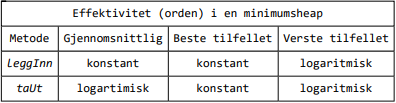
\includegraphics[center]{t-5.3.2-1.png}

    \subsection{5.3.3 Heap som prioritetskø}
        En minimumsheap kan (som et turneringstre) representeres ved hjelp av en tabell. 
        Indekser svarer til nodeposisjoner. 
        I algoritmene for å legge inn en verdi og å ta ut den minste verdien i
        en minimumsheap (se Avsnitt 5.3.2) var det nødvendig å kunne gå i begge retninge i treet,
        og det gjør vi ved hjelp av indeksene. 


    \subsection{5.3.6 Heapsortering}
        En tabell kan sorteres ved at den først gjøres om til en maksimumsheap og så gjøres den om til
        en sortert tabell. En slik algoritme kalles heapsortering.
        Når verdiene allerede ligger i en tabell, må også tabellelementet med indeks lik 0 være med.
        Det betyr at når tabellen skal «tolkes» som et komplett binærtre, må roten ha posisjon 0.

        Når rotnoden har posisjon 0, må vi bruke en annen regel enn før når det gjelder forelder og
        barn. Hvis en node nå har posisjon k, så vil venstre barn ha posisjon 2k + 1, høyre barn
        posisjon 2k + 2 og forelder posisjon (k - 1)/2. Dermed får en verdi samme indeks i tabellen som den har posisjon i treet.
        

\section{5.4 Huffmantrær}
    \subsection{5.4.1 Datakomprimering}
        Et Huffmantre er et fullt binærtre med spesielle egenskaper og brukes i
        forbindelse med komprimering av data.

    \paragraph{Kanonisk Huffmantre}
    \begin{enumerate}
        \item På samme nivå må nodene være sortert.
        \item Bokstavnodene må alltid være bladnoder.
        \item Veien ned til neste nivå må alltid gå via venstrebarnet.
    \end{enumerate}

        \paragraph{Bitmengder og størrelse}
        En vanlig bokstav representeres normalt med en binærkode på 8 biter (en byte). Bokstaven A
        har binærkoden 01000101. For å lagre informasjonen i
        den gitte sekvensen på 100 bokstaver brukes det en byte for hver bokstav, dvs. 100 byter og
        siden hver byte består av 8 biter, blir det tilsammen 800 bite

    \subsection{5.4.3 Huffmans metode}
        \paragraph{Oppsummert går Huffmans algoritme slik}
            \begin{enumerate}
                \item Gitt at vi kjenner frekvensen (antall forekomster) til hvert av de forskjellige tegnene i
                    en «melding». Disse tegnene omtales også som meldingens «alfabet».
                \item Lag en node for hvert av tegnene med tegnets frekvens som nodens frekvens og tegnet
                    som nodens tegn. Se Figur 5.4.3 a).
                \item Velg noden med minst og så den med nest minst frekvens. Hvis det er flere med minst
                    frekvens, er rekkefølgen likegyldig. Lag en ny node der den første blir venstre og den
                    andre høyre barn. Den nye nodens frekvens settes til summen av frekvensene til de to
                    som ble valgt ut. Tegnet i den nye noden har ikke interesse og kan være hva som helst.
                \item Den nye noden legges sammen med de andre. Det betyr at antallet i samlingen av
                    noder har blitt én mindre enn før (to tas ut, en legges inn). Se Figur 5.4.3 b) .
                \item Gjenta punkt 3. og 4. Se Figur 5.4.3 c) og Figur 5.4.3 d) .
                \item Når det er to noder igjen, vil den nye noden vi lager bli rotnode i Huffmantreet.
                    Frekvensen i noden blir lik antallet tegn i «meldingen». Se Figur 5.4.3 e) .
                \item Vi finner bitkoden for et tegn ved å starte i rotnoden og gå ned til tegnets node. En
                    0-bit til venstre og en 1-bit til høyre.
            \end{enumerate}

\newpage

    \subsection{5.4.4 Huffmanskogen og kanoniske trær}

        \paragraph{Huffmanskogen} Alle prefikskodetrær som har de samme tegnene og for hvert
        tegn samme avstand til roten som i et Huffmantre T, utgjør Huffmanskogen til T.

        \paragraph{Kanonisk tre} Det treet K i Huffmanskogen til et Huffmantre T som har alle
        nivåene fylt opp med noder fra venstre og med tegn på samme nivå sortert
        alfabetisk, kalles det (venstreorienterte) kanoniske treet. Hvis X og Y er to tegn i
        K, vil X alltid ligge til venstre for Y hvis X har større avstand fra roten enn Y eller
        hvis de har samme avstand og X kommer foran Y alfabetisk.

        \paragraph{Flg. regel gir antallet noder på hvert nivå. Verdiene i Tabell 5.4.4 b) brukes som eksempel: }
        \begin{enumerate}
            \item La n være størst bitkodelengde. Nivå n blir da nederste nivå. I vårt eksempel: n = 4.
            \item Nederste nivå skal ha noder, i alfabetisk rekkefølge, for de tegnene som har lengde n.
            Antallet slike er alltid et partall. I vårt eksempel er det C og G.
            \item La k < n. På nivå k får vi først foreldrene til de på nivå k + 1. Antallet blir halvparten av
            antallet noder på nivå k + 1. I tillegg kommer en node for hvert tegn som har lengde lik
            k. Antallet vil alltid bli et partall. Vårt eksempel: Antall noder på nivå 3 (k = 3) blir 2/1
            + 5 = 6 (2 noder på nivå 4 og 5 tegn med bitkodelengde lik 3). 
        \end{enumerate}

        \paragraph{Komprimering} Vi utvider nå Huffmans algoritme for å komprimere en «melding» til å bestå
        av følgende skritt:
            \begin{enumerate}
                \item Finn tegnene og frekvensfordelingen i «meldingen» som skal komprimeres.
                \item Finn Huffmantreet og så det tilhørende (venstreorienterte) kanoniske treet.
                \item Sett opp bitkodene som det kanoniske treet gir.
                \item Den komprimerte meldingen skal bestå av a) informasjon om tegnene og lengdene på
                    bitkodene og b) av at hvert tegn i «meldingen» er erstattet med sin bitkode.
            \end{enumerate}

        \paragraph{Dekomprimering} Den komprimerte meldingen behandles i motsatt rekkefølge:
            \begin{enumerate}
                \item Hent tegnene og bitkodelengdene.
                \item Sett opp det (venstreorienterte) kanoniske treet.
                \item Bitene bestemmer veien fra rotnoden og ned til et tegn (en bladnode).
            \end{enumerate}


\newpage
\part{Kapittel 6: Hashing og hashingteknikker}

\section{6.1 Hashing}

    \subsection{6.1.1 Hva er hashing?}
        I databehandling er hashing en teknikk for å legge objekter i en tabell på en slik måte at både
        innlegging, søking og fjerning blir effektive operasjoner. Målet er at alle tre operasjonene skal
        være av konstant orden. Teknikken består normalt av tre trinn:
        \begin{enumerate}
            \item Objektet deles opp ("hakkes i biter") og delene brukes til å konstruere et (stort) heltall.
                Dette heltallet kalles objektets hashverdi.
            \item Hashverdien (heltallet) konverteres ved hjelp av en bestemt regel til en tabellposisjon,
                f.eks. ved å bruke resten når hashverdien heltallsdivideres med tabellengden.
            \item  Hvis tabellposisjonen allerede er i bruk (kollisjon - et annet objekt ligger der), skal det
                likevel være mulig (ved hjelp av en fast regel) å lagre objektet og da på en slik måte at
                det lett kan gjenfinnes. Dette kalles kollisjonsbehandling.
        \end{enumerate}

        \begin{multicols}{2}
            Hashing er en så viktig teknikk at de som konstruerte Java valgte å la basisklassen Object få
            metoden hashCode(). Den er satt opp slik i klassen Object:

            \columnbreak
            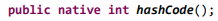
\includegraphics{k-6.1.1a.png}

        \end{multicols}

        \paragraph{Definisjon - Tetthet}
        Tettheten er er forholdet mellom antall elementer og lengden på tabellen. \\
        Definert som $\frac{antall}{dimensjon}$

        Et primtall som dimensjon gir best spredning.

        Kan se ut som om 75\% er en vanlig tetthetsgrense.

        Hvis vi setter grense (en heltallsvariabel) lik tetthet
        ganget med tabelldimensjon, kan antall sammenlignes med grense. Da sammenlignes to
        heltall og det er «billigere» enn å sammenligne to desimaltall.

    \subsection{6.1.2 Perfekte hashfunksjoner}
        \paragraph{Definisjon - Perfekt Hashfunksjon}

        La U være en universalmengde og A en delmengde av U med
        n verdier, N de naturlige tallene og B tallene fra 0 til n - 1. En perfekt
        hashfunksjon på A er en funksjon f : U → N som er en-til-en når den restrikteres
        til A. En minimal perfekt hashfunksjon på A er en funksjon f : U → B som er
        en-til-en når den restrikteres til A.

    \subsection{6.1.3 Generelle hashfunksjoner}
        Oppskriften sier at en hashfunksjon skal returnere et heltall som så skal brukes til å
        konstruere en indeks for lagringstabellen. Hvis vi kjenner de verdiene som det er aktuelt å
        lagre, kunne begge disse delene gjøres i ett (først et heltall og så en indeks). Et eksempel på
        dette kommer i forbindelse med LZW-metoden for komprimering. Se Avsnitt 7.2.6. Men hvis
        vi skal gjøre det generisk, må det gjøres i to operasjoner. Det betyr at instanser (objekter av
        datatypen) som det er aktuelt å lagre, må kunne "omformes" til et heltall. Deretter blir det
        hashsystemet (tabellstruktur og kollisjonsbehandling) som bruker dette heltallet. Slik er den
        generiske måten i Java.

        \subsubsection{Integer}
            Integer I Java arver som nevnt i Avsnitt 6.1.1, enhver klasse metoden hashCode() fra
            basisklassen Object. Den er overstyrt (eng: overridden) i alle Javas vanlige referansetyper,
            f.eks. Integer og String. I Integer returnerer den instansen verdi. Se flg. eksempel:

            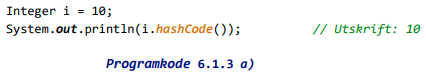
\includegraphics[center]{pk-6.1.3a.png}

            \begin{multicols}{2}
                Denne metoden, som til et tall tilordner det samme tallet, er en perfekt hashfunksjon. Det
                kan imidlertid være gunstig å gjøre en primtallsbasert forskyvning. Klassen Heltall er et
                eksempel på en «omslagsklasse» (for datatypen int). Den er laget på samme måte som
                Integer. Hvis vi ikke koder hashCode() og equals() i Heltall, vil både NetBeans og Eclipse
                foreslå hvordan de skal kodes. NetBeans kommer med flere forslag. Et av dem er som følger
                (der verdi er instansvariabelen i klassen):
                \columnbreak
                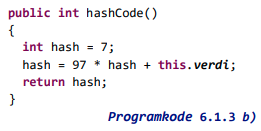
\includegraphics[center, scale=1.2]{pk-6.1.3b.png}
            \end{multicols}

            \hrule width \textwidth

            \begin{multicols}{2}
                I Eclipse kommer det kun ett forslag og det ser slik ut:

                Begge versjonene gir en perfekt hashfunksjon siden,
                funksjonsverdien er forskjøvet en fast verdi i forhold til argumentet.

                \columnbreak
                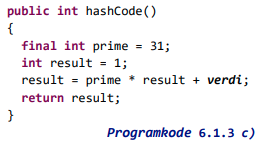
\includegraphics[center]{pk-6.1.3c.png}
            \end{multicols}

        \subsubsection{Double}

    \subsection{6.1.4 Lukket adressering}
        \paragraph{Lukket adressering} betyr at ved kollisjon skal objektet legges inn på den indeksen vi
        fikk. Men da må vi ha en datastruktur som tillater flere objekter på samme indeks.

        \paragraph{Innlegging}
        \begin{enumerate}
            \item Lag en ny node som inneholder objektet.
            \item Finn objektets tabellindeks indeks.
            \item Sjekk hash[indeks].
            \item Hvis den er null, la den referere til den nye noden.
            \item Hvis den ikke er null, la den nye noden bli første node i den tilhørende listen.
            \item Øk antallvariabelen.
        \end{enumerate}

        \paragraph{Søking}
        \begin{enumerate}
            \item Finn tabellindeksen.
            \item Søk i den (eventuelt tomme) (lenkede) listen som
                hører til indeksen.
            \item Hvis objektet ikke ligger der, så finnes ikke objektet.
        \end{enumerate}

        \paragraph{Fjerning}
        \begin{enumerate}
            \item Finn tabellindeksen.
            \item Søk i den (eventuelt tomme) (lenkede) listen som
                hører til indeksen.
            \item Fjern den (hvis den er der) på vanlig måte (ved å endre på en
                referanse).
            \item Reduser antallvariabelen.
        \end{enumerate}

\newpage
\part{Kapittel 9: Balanserte binærtrær}

\section{9.2 Rød-svarte og 2-3-4 trær}
    \subsection{9.2.1 B-tre av orden 4 eller 2-3-4 tre}
        Et 2-3-4 tre (et B-tre av orden 4) og et rød-svart tre er to ekvivalente datastrukturer. Et
        2-3-4 tre kan omformes til et rød-svart tre og omvendt, et rød-svart tre kan omformes til et
        2-3-4 tre. Rød-svarte trær er mest brukt, f.eks. i klassene TreeSet og TreeMap i java.util. I
        et 2-3-4 tre må noder kunne «splittes» når treet bygges opp og det er litt komplisert å kode
        på grunn av mange spesialtilfeller. I et rød-svart tre brukes «farger» og rotasjoner og det er
        enklere å kode. Men det er imidlertid enklere å forstå hva som skjer i et 2-3-4 tre og hvorfor
        det blir balansert. Derfor kan det pedagogisk sett være lurt å starte med 2-3-4 trær og så gå
        over til rød-svarte trær når en har forstått idéene.

        Et 2-3-4 tre er ikke et binærtre. Det er et balansert tre der nodene kan ha flere enn to barn. I
        et binærtre kan en node ha ingen, ett eller to barn. Generelt gjelder at i et B-tre av orden m
        kan en node ha maksimalt m barn. En node kan der ha ingen barn (en bladnode), men aldri
        kun ett barn. I et B-tre av orden 4 kan dermed en indre node ha 2, 3 eller 4 barn. Derfor
        kalles det også et 2-3-4 tre. For et slikt tre gjelder:
        \begin{enumerate}
            \item En node kan ha én, to eller tre verdier. En node med én verdi kalles en 2-node, en med
                  to verdier kalles en 3-node og en med tre verdier en 4-node.
            \item En indre node kan ha to, tre eller fire barn.
            \item Antallet verdier i en indre node er alltid én mindre enn antallet barn som noden har.
            \item Alle bladnoder ligger på samme nivå i treet.
        \end{enumerate}

        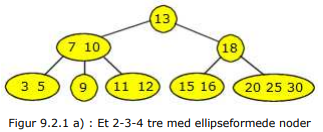
\includegraphics[center]{f-9.2.1a.png}

        \subsubsection{Sorteringsorden}
            I en node med flere verdier skal verdiene være sortert (stigende). I slike
            trær kan vi imidlertid ikke, som for binære trær, snakke om en nodes venstre og høyre subtre
            siden det kan være 2, 3 eller 4 subtrær. Men for hver verdi i en indre node kan vi snakke om
            dens venstre og høyre subtre. Se på noden med verdiene 7 og 10 i Figur 9.2.1 a): Vi kan si
            at verdien 7 har to subtrær - det venstre består av noden med verdiene 3 og 5 og det høyre
            av noden med verdien 9. På samme måte har verdien 10 to subtrær - det venstre består av
            noden med verdien 9 og det høyre av noden med verdiene 11 og 12. Dette betyr spesielt at
            noden/subtreet med verdien 9 er høyre subtre til 7 og venstre subtre til 10.
            Sorteringsrekkefølgen for verdiene i et 2-3-4 tre blir dermed slik:
                \begin{enumerate}
                    \item Verdiene i hver node skal være sortert stigende.
                    \item Hvis x er en vilkårlig verdi i en indre node, skal største verdi i det venstre subtreet til x
                    være mindre enn x, og x skal være mindre enn minste verdi i høyre subtreet til x.
                \end{enumerate}


            Vi ser i Figur 9.2.1 a) at rotnoden har verdien 13, at alle verdiene i dens venstre subtre er
            mindre enn 13 og alle verdien i det høyre er større enn 13, osv. Sorteringsrekkefølgen blir
            dermed som forventet lik 3, 5, 7, 9, 10, 11, 12, 13, 15, 16, 18, 20, 25, 30. 

        \paragraph{Definisjon - Selvbalanserende tre}
        Prøver å få søketreet "mer" perfekt.


    \subsection{9.2.2 Innlegging og søking i et 2-3-4 tre}
        \subsubsection{Innleggingsalgoritme (ovenifra og ned) for 2-3-4 trær}
            \begin{enumerate}
                \item Hvis treet er tomt, opprettes en bladnode og verdien legges inn i den.
                \item Finn den bladnoden som verdien sorteringsmessig hører til. Splitt alle 4-noder som
                    passeres på veien ned dit (også bladnoden hvis den er en 4-node). En node splittes ved
                    at midtverdien rykker opp til foreldernoden (på rett sortert plass) og ved at de to
                    verdiene på hver siden inngår i sine egne noder. Hvis det er rotnoden som skal splittes,
                    rykker midtverdien opp til en ny rotnode.
                \item Hvis bladnoden har plass, legges verdien inn på rett sortert plass. Hvis den ble splittet
                    (var en 4-node), legges verdien inn i den noden som den etter splittingen hører til.
            \end{enumerate}

            \paragraph{Søking} i et 2-3-4 tre er rett frem. Det er bare å bruke sorteringsrekkefølgen. Start i rotnoden
            og gå eventuelt videre til et barn basert på størrelsen på søkeverdien i forhold til
            nodeverdiene. Hvis en kommer til en bladnode og skal videre, er ikke verdien i treet.



    \subsection{9.2.4 Fra 2-3-4 tre til rød-svart tre}
        I et rød-svart tre har nodene to farger. I et vanlig binærtre vil venstre og/eller høyre peker i
        en node kunne være null. Her skal vi isteden si at den peker til en svart "nullnode".
        \paragraph{Et rød-svart tre (eng: red-black tree) er definert på følgende måte}
        \begin{multicols}{2}
            \begin{enumerate}
                \item Det er et binært søketre der det normalt ikke er tillatt med like verdier.
                \item Nodene er enten røde eller svarte. Rotnoden er svart.
                \item Barna til en rød node er svarte.
                \item Pekere som i et vanlig tre peker til null, skal her isteden peke til en svart "nullnode".
                \item La p være en vilkårlig node. Da er antall svarte noder på veien mellom p og en nullnode
                    i subtreet med p som rot, det samme for alle slike nullnoder.
            \end{enumerate}

            \columnbreak

            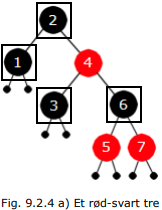
\includegraphics[scale=0.8, center]{figur-9.2.4a.png}
        \end{multicols}

        \paragraph{Omregningsformler}
        \begin{multicols}{2}
            \begin{enumerate}
                \item \textbf{Formel 1:} En 2-node i et 2-3-4 tre med verdi x "oversettes" til en svart node med verdi
                    x i et rød-svart tre.
                \item \textbf{Formel 2:} En 3-node i et 2-3-4 tre med verdiene x og y "oversettes" enten til
                    \begin{enumerate}[a), itemsep=0.5mm]
                        \item En svart foreldernode med verdi x og et rødt høyre barn med verdi y
                        \item[] eller
                        \item En svart foreldernode med verdi y og et rødt venstre barn med verdi x
                    \end{enumerate}
                \item \textbf{Formel 3:} En 4-node i et 2-3-4 tre med verdiene x, y og z "oversettes" til en svart
                    foreldernode med verdi y, et rødt venstre barn med verdi x og et rødt høyre barn med
                    verdi z.
            \end{enumerate}
            \columnbreak
            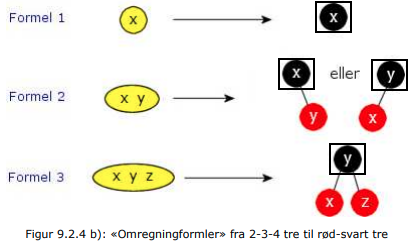
\includegraphics[scale=0.9]{figur-9.2.4b.png}
        \end{multicols}

\newpage

        \paragraph{Eksempel}

        I følgende eksempel skal vi "oversette" 2-3-4 treet i Figur 9.2.4 c) under :\\

        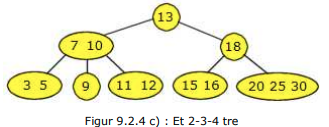
\includegraphics[center]{figur-9.2.4c.png}

        Siden 2-3-4 treet har en rotnode med kun én verdi blir den gjort om til en svart nullnode i det
        rød-svarte treet. Det venstre barnet til rotnoden i 2-3-4 treet har to verdier, dvs at det er en
        3-node.
        Da kan vi bruke enten a) eller b) i Formel 2. Valget vil påvirke treets utseende, men
        trærne blir likeverdige. Her velger vi å bruke muligheten a) for alle 3-noder. Vi ser senere på
        hvordan treet vil bli hvis vi f.eks. isteden bruker b) for alle 3-noder. Det er også mulig å
        blande, dvs. noen ganger a) og noen ganger b). Resultatene blir likeverdige.

        \begin{multicols}{2}
            Noden med verdiene 7 og 10 skal derfor gjøres om til en svart foreldernode (som blir venstre
            barn til roten) med verdi 7 og et rødt høyre barn til den med verdi 10. Osv. Resultatet blir:
            \columnbreak
            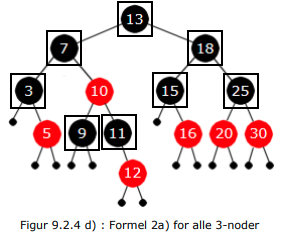
\includegraphics[center]{figur-9.2.4d.png}
        \end{multicols}



        Algoritmen for å "oversette" et 2-3-4 tre til et rød-svart tre er, som nevnt over, ikke entydig.
        Formel 2 sier at vi kan omskape en 3-node (som har to verdier) til to noder der enten
        \begin{enumerate}[nosep]
            \item Første verdi legges i en svart foreldernode og den andre verdien i et rødt høyrebarn.
            \item[] eller
            \item At første verdi legges i et rødt venstrebarn og den andre verdien i en svart forelder.
        \end{enumerate}

        \begin{multicols}{2}
            Men alle trær får samme høyde og samme svarte høyde.
            Treet i \emph{Figur 9.2.4 d)} ble til ved at \textbf{a)} ble brukt i alle tilfellene.
            Hvis vi isteden velger å bruke \textbf{b)} i alle tilfellene, får vi flg. tre:

            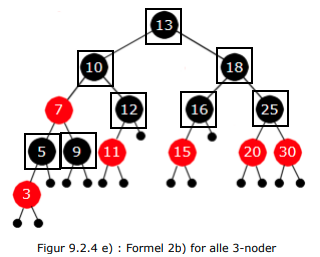
\includegraphics[center]{figur-9.2.4e.png}
        \end{multicols}

\newpage

    \subsection{9.2.5 Innlegging i et rød-svart tre}
        \paragraph{Innleggingsalgoritmen}
        \begin{enumerate}
            \item Treets første verdi legges i en svart rotnode.
            \item  Generelt legges en ny verdi i en rød node på rett sortert plass i treet. La den hete X.
            \item Hvis forelder F til X er svart, stopper vi. Hvis F er rød, må F ha en svart forelder B
                (besteforelder til X) og X en tante T (søsken til forelder F).
            \item Hvis T er svart (en nullnode eller en vanlig node), er det fire mulige tilfeller. Avhengig
                av hviklet tilfelle det er (se huskereglene over) må det utføres en enkel eller en dobbel
                rotasjon (høyre eller venstre) og deretter et fargeskifte (F til svart og B til rød). Dermed
                er innleggingen ferdig.
            \item Hvis T er rød, må det utføres et fargeskifte (F og T til svart og B til rød). Hvis B er
                roten, settes den tilbake til svart og vi kan stoppe. Hvis ikke, omdøper vi B til X og går
                tilbake til pkt. 3.
        \end{enumerate}

        \paragraph{Eksempel}
        Vi skal fortløpende legge inn tallene 1, 2, 3, 4, 5, 6, 7 og 8. I et vanlig
        binært søketre ville det ha resultert i et ekstremt høyreskjevt tre.
        Men her skal vi se (etter en del arbeid underveis) at det blir et balansert tre. \\

        \hrule width \textwidth

        \begin{multicols}{2}
            Den første verdien (dvs. tallet 1) legges i en svart rotnode:

            \columnbreak
            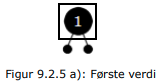
\includegraphics[center]{f-9.2.5a.png}
        \end{multicols}

        \hrule width \textwidth

        \begin{multicols}{2}
            Deretter gjør vi som i et vanlig binært søketre.
            Verdien (dvs. 2) legges på rett sortert plass i treet.
            En ny node skal alltid være rød. Her blir den nye noden høyre barn til rotnoden:

            Vi må sjekke om treet oppfyller definisjonen til et rød-svart tre. Algoritmen er heldigvis laget
            slik at det er kun punkt 3 som må sjekkes: En rød node kan ikke ha et rødt barn. Eller
            omvendt: En rød node kan ikke ha en rød forelder. Treet i Figur 9.2.5 b) er derfor ok.

            \columnbreak
            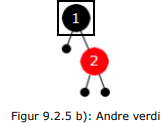
\includegraphics[center]{f-9.2.5b.png}
        \end{multicols}

        \hrule width \textwidth

        \begin{multicols}{2}
            Neste verdi, dvs. tallet 3, legges først på rett sortert plass i en rød node:

            \columnbreak
            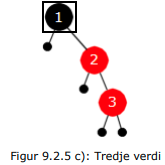
\includegraphics[center]{f-9.2.5c.png}
        \end{multicols}

        \hrule width \textwidth

        Treet i Figur 9.2.5 c) er i strid med punkt 3 i definisjonen (rød node har rød forelder). Legg
        merke til at hvis vi hadde lagt inn de tre verdiene 1, 2 og 3 i en annen rekkefølge, ville treet
        ha blitt annerledes. De seks permutasjonene av 1, 2 og 3 vil gi flg. fem forskjelige tilfeller:

        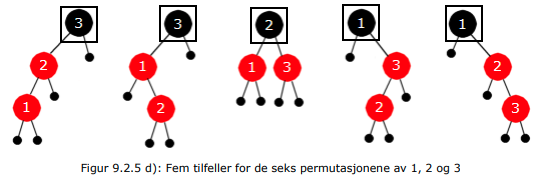
\includegraphics[center]{f-9.2.5d.png}

        \hrule width \textwidth

        Rekkefølgen 2,1,3 og 2,3,1 gir det midterste treet i Figur 9.2.5 d). Det treet er ok. Men alle
        de fire andre trærne er i strid med punkt 3 i definisjonen. Det er en separat regel for hvert av
        de fire tilfellene. Her fortsetter vi imidlertid med treet i Figur 9.2.5 c). For å forklare dette
        grundig gir vi nodene navn som om det var et lite familietre.

        \begin{multicols}{2}
            Den nye noden (det nye barnet)
            får navnet X siden dens endelige plassering foreløpig er ukjent. Dens forelder får navnet F,
            dens besteforelder B og dens «tante» T (tante siden noden T er søsken til forelder F):

            \columnbreak
            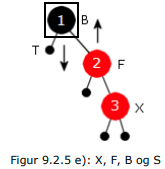
\includegraphics[center]{f-9.2.5e.png}
        \end{multicols}

        \hrule width \textwidth

        \begin{multicols}{2}
            I Figur 9.2.5 e) er T svart, F er høyre barn til B og X høyre barn til F. Dette «repareres» ved
            hjelp av venstrerotasjon og fargeskifte. Vi roterer treet mot venstre om midtpunktet på
            kanten mellom B og F. Det fører til at noden F heves (pil oppover) og noden B senkes (pil
            nedover). Deretter skifter de to farge - F blir svart og B blir rød. Etterpå fjernes navnene X, F,
            B og T siden de ikke lenger gir mening:

            \columnbreak
            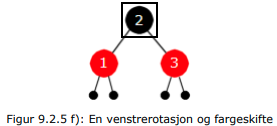
\includegraphics[center]{f-9.2.5f.png}
        \end{multicols}

        \hrule width \textwidth

        \begin{multicols}{2}
            Neste verdi er 4 og den legges som normalt på rett sortert plass, dvs. som høyre barn til
            3-noden. En ny node er alltid rød. Vi setter igjen navn på nodene. Den nye heter X, osv:

            \columnbreak
            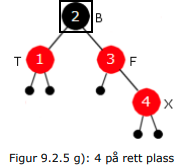
\includegraphics[center]{f-9.2.5g.png}
        \end{multicols}

        \hrule width \textwidth

        \begin{multicols}{2}
            Treet i Figur 9.2.5 g) er «ulovlig» siden X og F er røde. Denne gangen er T rød. De fire
            tilfellene med rød T er de enkle tilfellene. Alle «repareres» på samme måte, dvs. ved kun å
            skifte farger: F og T blir svarte og B blir rød. Men siden B her er roten, settes den tilbake til
            svart. Roten skal alltid være svart. Hvis B ikke var roten, kunne vi ha fått et nytt problem.
            Forelderen til B kunne jo være rød og da får vi rødt barn med rød forelder. Et slikt tilfelle
            dukker opp når vi skal legge inn 8. Se lenger ned. Treet blir slik:

            \columnbreak
            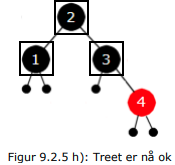
\includegraphics[center]{f-9.2.5h.png}
        \end{multicols}

        \hrule width \textwidth

        \begin{multicols}{2}
            Neste verdi er 5 og den legges som vanlig i en rød node på rett sortert plass:

            \columnbreak
            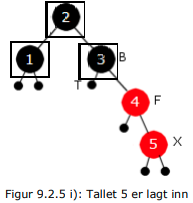
\includegraphics[center]{f-9.2.5i.png}


        \end{multicols}

        \hrule width \textwidth

        \begin{multicols}{2}
            Vi får samme tilfelle som i Figur 9.2.5 e) og «reparerer» på samme måte - en venstrerotasjon
            og et fargeskifte. Her må vi imidlertid passe på at høyrepeker i 2-noden settes riktig:

            \columnbreak
            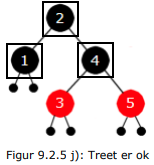
\includegraphics[center]{f-9.2.5j.png}


        \end{multicols}

        \hrule width \textwidth

        Når 6 legges inn vil vi få at X, F er T røde. Det er, som nevnt over, et enkelt tilfelle, dvs. kun
        et fargeskifte: F og T blir svarte og B blir rød:

        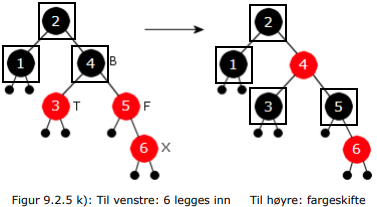
\includegraphics[center]{f-9.2.5k.png}


        \hrule width \textwidth

        \begin{multicols}{2}
            Når 7 legges inn ser vi at vi får det samme tilfellet som i Figur 9.2.5 e) en gang til. Dermed
            en venstrerotasjon og et fargeskifte:

            \columnbreak
            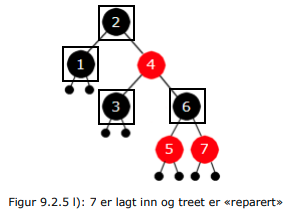
\includegraphics[center]{f-9.2.5l.png}


        \end{multicols}

        \hrule width \textwidth

        Siste verdi er 8. Den legges som vanlig i en rød node på rett sortert plass. Da får vi det
        venstre treet i figuren under. Her er T rød og da blir det fargeskifte: F og T blir svarte og B
        blir rød. Det gir treet til høyre i figuren under:

        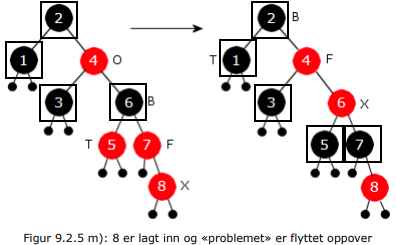
\includegraphics[center]{f-9.2.5m.png}

        \hrule width \textwidth

        \begin{multicols}{2}
            Men nå har vi fått et nytt problem. Siden oldeforelder O til X (forelder til B) er rød, får vi et
            tilfelle som er strid med punkt 3 i definisjonen. Dvs. rød node med rød forelder. I treet til
            høyre i figuren over er navnsettingen X, F, T og B flyttet oppover slik at de to røde nodene
            heter X og F. Men dette er en kjent tilfelle siden T nå er svart. Det betyr en venstrerotasjon
            og fargeskifte. Vi roterer om B - F (midpunktet på kanten mellom B og F). Det betyr at F
            heves og B senkes. Spesielt blir venstre subtre til F etterpå høyre subtre til B. Etter
            rotasjonen settes B til rød og F til svart. Dermed får vi (etter at navnene (bokstavene) er
            fjernet) dette vakre resultatet:


            \columnbreak
            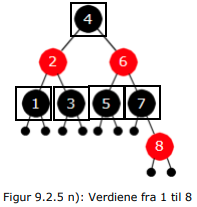
\includegraphics[center]{f-9.2.5n.png}

        \end{multicols}

        \hrule width \textwidth

        \begin{multicols}{2}
            Ved innlegging av tallene fra 1 til 8 har kun to av de åtte tilfellene (der F og X er røde)
            oppstått. Vi skiller mellom hovedtilfellene T svart (fire tilfeller) og T rød (fire tilfeller).
            Som nevnt over er tilfellene med rød T enkle å behandle. Da er det kun fargeskifte - F og T blir
            svarte og B rød. Men som vist over (innlegging av 8) kan det føre til «problemer» oppover i
            treet. Det skjer hvis oldeforelder til X er rød. Da flyttes «navnene» X, F, T og B oppover og
            det nye tilfellet «repareres». Osv.
            Hvis T derimot er svart, blir det rotasjoner og fargeskifte. Men da stopper det siden det da
            aldri blir rød node med rød forelder. Figur 9.2.5 d) viser de fem trærne som oppstår ved å
            legge inn tallene 1, 2 og 3 i en eller annen rekkefølge. Spesielt får vi dette treet hvis vi legger
            inn i rekkefølgen 1, 3, 2:


            \columnbreak
            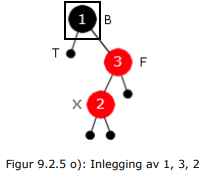
\includegraphics[center]{f-9.2.5o.png}

        \end{multicols}

        \hrule width \textwidth

        Forskjellen mellom denne og den i Figur 9.2.5 e) er at nodene B - F - X nå danner en «knekk»
        eller en vinkel, mens nodene i Figur 9.2.5 d) går på skrå (ned mot høyre). Her «reparerer» vi
        ved å heve noden X to nivåer oppover og senke B ett nivå nedover. Deretter blir X svart og B
        rød. Dette kalles en dobbel venstrerotasjon med fargeskifte siden resultatet oppnås ved to
        rotasjoner. Først roterer vi mot høyre mhp. F - X, dvs. om midtpunktet på kanten mellom F
        og X. Da heves X og F senkes. Deretter (vi beholder nodenavnene) roterer vi mot venstre
        mhp. B - X. Flg. sekvens viser hva som skjer:


        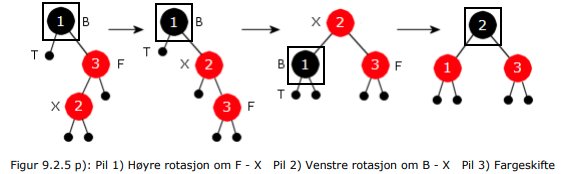
\includegraphics[center]{f-9.2.5p.png}

        \hrule width \textwidth

        \textbf{Huskeregler med illustrasjoner}

        Hvis vi har det «ulovlige» tilfellet rød node med rød forelder, kaller vi noden X, dens forelder
        F, dens tante (søsken til forelder) T og dens besteforelder B. Vi har to hovedtilfeller: T er
        svart og T er rød.

        Hvis T er svart trengs en rotasjon (og et fargeskifte). Ved en rotasjon kan et eller to subtrær
        bytte «eier». Det eller de dette gjelder er i tegningene under markert med en blå node. Et
        slikt subtre kan være både tomt og ikke tomt. Hvis det er tomt svarer det til en nullnode.

        \textbf{1) T er svart, B - F - X ligger på skrå (to tilfeller)}

        \textbf{1a)}
        B - F - X går på skrå ned mot høyre hvis F er høyre barn til B og X er høyre barn til F.
        Dette repareres ved en venstrerotasjon mhp. B - F (F heves og B senkes) og et fargesifte (B
        blir rød og F svart). Venstre subtre til F (symbolisert med en blå node) blir høyre subtre til B.

        \textbf{1b)}
        B - F - X går på skrå ned mot venstre hvis F er venstre barn til B og X er venstre barn til
        F. Dette repareres ved en høyrerotasjon mhp. B - F (F heves og B senkes) og et fargesifte (B
        blir rød og F svart). Høyre subtre til F (symbolisert med en blå node) blir venstre subtre til B.

        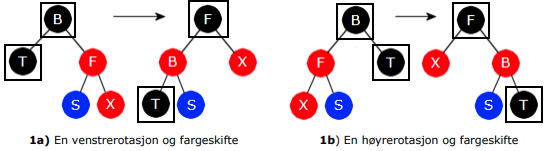
\includegraphics[center]{f-9.2.5-1ab.png}



        \textbf{2) T er svart, B - F - X har en knekk (to tilfeller)}

        \textbf{2a)}
        B - F - X har en «knekk» (eller vinkelspiss) mot høyre hvis F er høyre barn til B og X er
        venstre barn til F. Dette repareres ved en dobbel venstrerotasjon (X heves to nivåer og B
        senkes ett nivå) og et fargeskifte (B blir rød og X svart). Venstre subtre til X (symbolisert
        med den blå noden S1) blir høyre subtre til B og høyre subtre til X (symbolisert med den blå
        noden S2) blir venstre subtre til F.


        \textbf{2b)]} B - F - X har en «knekk» (eller vinkelspiss) mot venstre hvis F er venstre barn til B og X
        er høyre barn til F. Dette repareres ved en dobbel høyrerotasjon (X heves to nivåer og B
        senkes ett nivå) og et fargeskifte (B blir rød og X svart). Venstre subtre til X (symbolisert
        med den blå noden S1) blir høyre subtre til F og høyre subtre til X (symbolisert med den blå
        noden S2) blir venstre subtre til B.

        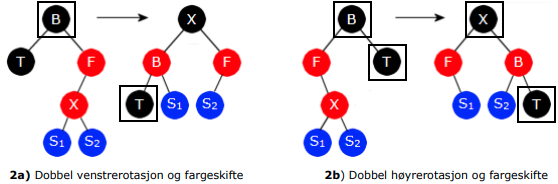
\includegraphics[center]{f-9.2.5-2ab.png}


\newpage

        \textbf{3) T er rød (fire tilfeller)}

        Dette er de enkle tilfellene. Alle sammen (fire tilfeller) behandles på samme måte. Dvs. et
        fargeskifte der B blir rød og F og T svarte. Men da kan det oppstå nye tilfeller oppover i treet.
        Hvis B har en forelder som er rød, vil både den og B etter fargeskiftet være røde. Da flyttes
        navnsettingen oppover ved at B settes til X, osv. Det en da får er et av de åtte mulige
        tilfellene og det behandles slik det tilfellet skal behandles.

        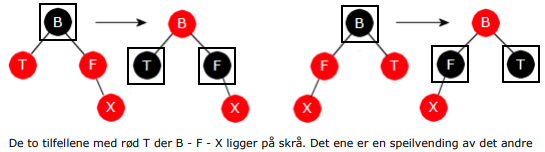
\includegraphics[center]{f-9.2.5-3.1.png}

        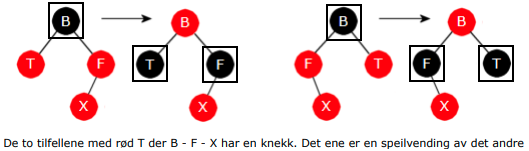
\includegraphics[center]{f-9.2.5-3.2.png}

\newpage
    \subsection{9.2.6 Java-kode for et rød-svart tre}
        Nodene i et rød-svart skal ha en farge. Til det brukes to fargekonstanter SVART og RØD. Vi
        trenger også «nullnoder». I realiteten lager vi kun én nullnode (en konstant) med navn NULL
        som alle da kan peke til. Klassen får navnet RSBinTre der R står for rød og S for svart:

        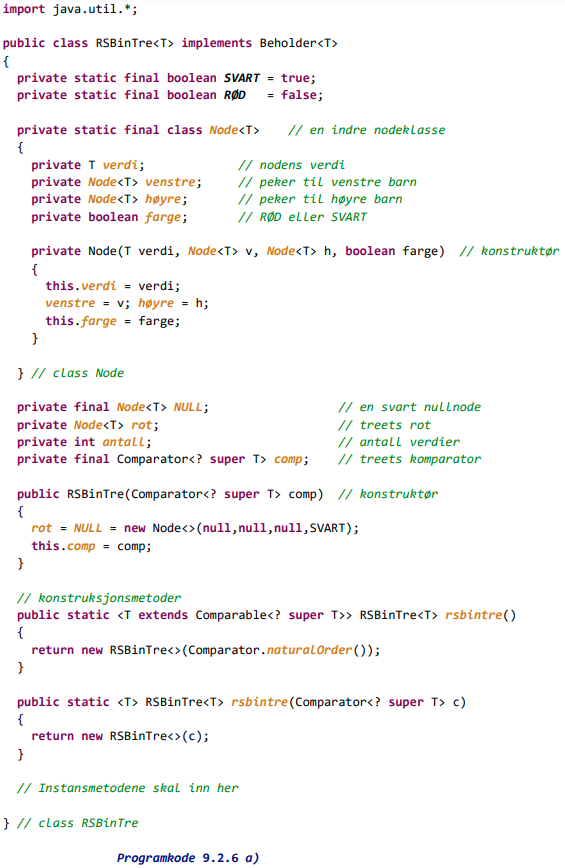
\includegraphics[center]{pk-9.2.6a.png}

        Flere av metodene fra klassen SBinTre kan brukes i klassen RSBinTre. Men pga. nullnoden
        NULL må vi gjøre noen små endringer. F.eks. slik i metoden inneholder(T verdi):

        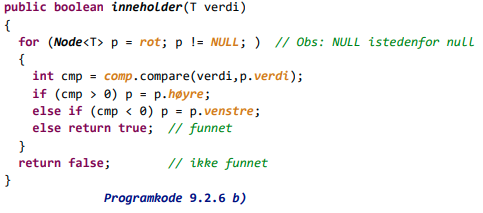
\includegraphics[center]{pk-9.2.6b.png}

        Utfordringen ligger i metoden leggInn(). Vi legger inn som i et vanlig binært søketre, men
        hvis treet må «repareres» etterpå, må vi kunne gå oppover. Det kan vi løse ved hjelp av en
        stakk. Alle nodene på veien nedover legges på stakken. Metoden starter derfor slik:

        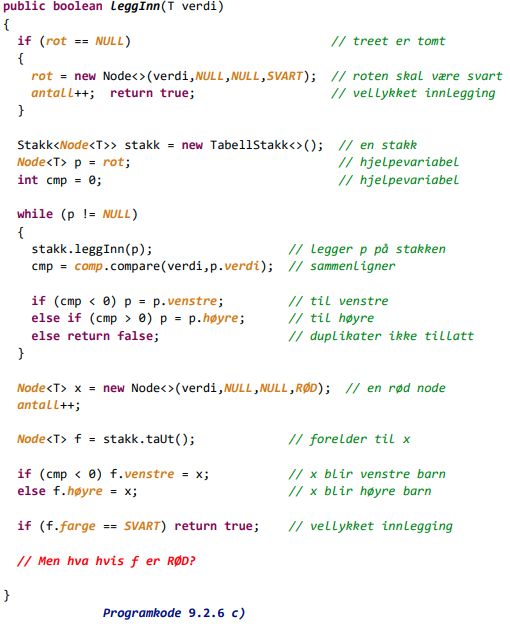
\includegraphics[center]{pk-9.2.6c.png}

        Så langt er Programkode 9.2.6 c) omtrent som for et vanlig binært søketre. Men hvis forelder
        f til x er rød, så blir det annerledes. I så fall kan ikke f være rotnoden siden den alltid er
        svart. Da må x ha en besteforelder b og den må da ligge øverst på stakken. Deretter må vi
        starte en løkke. I den finner vi først «tanten» t til x. Så må vi avgjøre om t er et venstre eller
        et høyre barn til b. Dvs. hvis f er er venstre barn til b, så må t være høyre barn og omvendt.
        Som beskrevet i reglene er det to hovedtilfeller: t svart eller t rød.

        Flg. kode skal inn der det står // Men hva hvis f er RØD? i Programkode 9.2.6 c):

        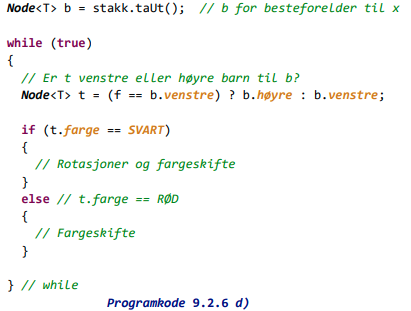
\includegraphics[center]{pk-9.2.6d.png}

        Hvis t.farge er SVART har vi fire undertilfeller - se reglene. I hver av dem inngår en enkel
        eller en dobbel rotasjon Doble rotasjoner består av to enkle rotasjoner. Koden for en generell
        enkel rotasjon er ikke vanskelig. Figuren under viser gangen i en venstrerotasjon på p - q:

        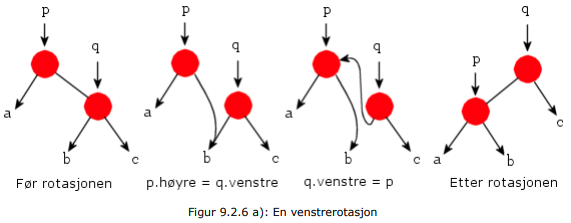
\includegraphics[center]{f-9.2.6a.png}

        Figuren viser gangen i en venstrerotasjon på p - q, dvs. p er forelder og q er høyre barn.
        Rotasjonen foregår om midtpunktet mellom p og q. Det fører til at p senkes og q heves og
        dette kun ved hjelp av de to programsetningene p.høyre = q.venstre og q.venstre = p. De
        to siste trærne i Figur 9.2.6 a) er like. Det siste er satt opp på en «penere» form.

        En høyrerotasjon er en speilvending av en venstrerotasjon og utføres på p - q (q er venstre
        barn til p) ved hjelp av setningene p.venstre = q.høyre og q.høyre = p. Vi setter dette opp
        i to metoder der p og q er argumenter:

        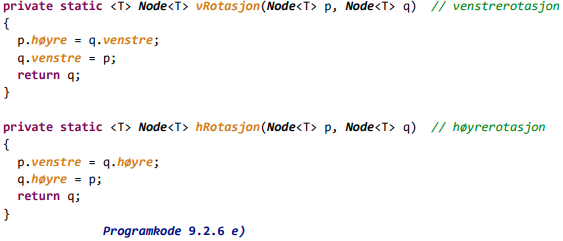
\includegraphics[center]{pk-9.2.6e.png}

        De fire tilfellene 1a), 1b), 2a) og 2b) fra reglene må behandles hver for seg. For å finne hvem
        av dem som er aktuelle, må vi undersøke om x er venstre eller høyre barn til f og om f er
        venstre eller høyre barn til b. I alle tilfellene skal b bli rød. Det gir flg. kode:

        En dobbel rotasjon utføres ved å kalle metodene over to ganger.

        \includegraphics[center]{pk-9.2.6f.png}

\newpage

        I tilfellet s.farge er RØD har vi også fire undertilfeller - se illustrasjonene. Men denne gangen
        trengs det kun å skifte farger:

        \includegraphics[center]{pk-9.2.6g.png}

        Vi kan sette sammen alt dette til en fullstendig kode for metoden leggInn(). Dette og kode
        for en del andre aktuelle metoder ligger på RSBinTre. Hvis du flytter hele klassen over til deg
        selv, vil du kunne kjøre flg. programbit:

        \includegraphics[center]{pk-9.2.6h.png}

\newpage
\part{Kapittel 11: Grafer}

\section{11.1 Uvektede grafer}
    \subsection{11.1.1 Generelt om grafer}
        En graf har noder (eng: node/nodes eller vertex/vertices) og kanter (eng: edge/edges)
        mellom dem. En kant er formelt et par av noder. Kanten kalles rettet hvis paret er ordnet
        og urettet hvis paret er uordnet. En graf tegnes vanligvis ved å la nodene være små sirkler
        og kantene streker mellom noder. En rettet kant tegnes normalt som en pil. En kant kan ha
        en vekt (eller lengde) i form av et tall. Vi skiller nodene fra hverandre ved å gi hver av dem
        et unikt «navn», dvs. en identifikator.

        \paragraph{Urettet og uvektet graf} Figur 11.1.1 b) under til venstre viser en urettet og uvektet graf
        med 7 noder og 12 kanter. Der brukes en bokstav som identifikator:

        \includegraphics[center]{f-11.1.1bc.png}

        \paragraph{Rettet og uvektet graf} En graf kalles rettet (eng: directed graph eller digraph) hvis alle
        kantene har en retning, dvs. at de er representert som ordnede par. Figur 11.1.1 c) over til
        høyre viser en rettet (og uvektet) graf. Den er laget ved at hver av kantene i grafen i Figur
        11.1.1 b) har fått retning. En vanlig måte å markere retning på er å bruke en pil.

        \paragraph{Urettet og vektet graf} En graf kalles vektet (eng: weighted) hvis det til hver kant er
        tilordnet en vekt (et tall). Verdien kalles generelt kantens vekt, men i mange situasjoner er
        det mer naturlig å si at det er kantens lengde. Grafen i Figur 11.1.1 d) under til venstre er
        urettet og vektet:

        \includegraphics[center]{f-11.1.1de.png}

        \paragraph{Rettet og vektet graf} Grafen i Figur 11.1.1 e) over til høyre er rettet og vektet:

\newpage

        \textbf{Oppsummering} \\

            Vi kan oppsummere dette ved å si at det er fire hovedtyper av grafer, men det er også grafer
            som er en kombinasjon av disse hovedtypene:

            1) Urettet og uvektet, 2) Rettet og uvektet, 3) Urettet og vektet og 4) Rettet og vektet.

            En kant er et nodepar. Hvis de to nodene i paret er like, kalles det en sløyfe (eng: loop). En
            graf uten sløyfer kalles sløyfefri. Det kan også være to eller flere like par, dvs. flere kanter
            mellom to noder. Det gir flg. graftyper:

            \begin{enumerate}
                \item Enkel urettet graf - maksimalt én kant mellom to noder og sløyfefri.
                \item Enkel rettet graf - maksimalt én kant i samme retning mellom to noder og sløyfefri.
                \item Multigraf - det kan være flere kanter mellom to noder, men sløyfefri.
                \item Pseudograf - det kan være flere kanter mellom to noder og noder kan ha sløyfer.
            \end{enumerate}

        \subsubsection{Urettet graf}
            Vi har blant andre flg. begreper:
            \begin{enumerate}
                \item \textbf{Nabo} To noder X og Y kalles naboer hvis det går en kant mellom dem. I Figur 11.1.1 b)
                    er A og B naboer, men ikke nodene A og E. Naboene til A er B, C og D. På engelsk er to
                    noder adjacent (tilstøtende) hvis de er naboer.
                \item \textbf{Nodegrad} Graden til en node er lik kantantallet. En sløyfe utgjør to kanter. F.eks. er
                    graden til A i Figur 11.1.1 b) lik 3 og den til D lik 6.
                \item \textbf{Vei og veilengde} Det går en vei mellom to noder X og Y hvis det er mulig å gå fra X
                    til Y ved å følge kanter. Hvis grafen er uvektet, er veilengden lik antallet kanter og hvis
                    den er vektet, er veilengden summen av kantvektene.
                \item \textbf{Enkel vei} En vei kalles enkel hvis alle kantene på veien er forskjellige.
                \item \textbf{Sykel} En enkel vei som starter i en node X, inneholder minst én kant og som ender der
                    den startet (dvs. i X ), kalles en sykel eller en krets (eng: circuit). En graf uten sykler
                    kalles asyklisk.
                \item \textbf{Korteste vei} Hvis det går flere enn én vei mellom to noder X og Y, er den veien
                    kortest som inneholder færrest kanter eller minst kantvektsum hvis grafen er vektet.
                \item \textbf{Sammenheng} Grafen kalles sammenhengende hvis det går en vei mellom hvert par av
                    forskjellige noder X og Y. Hvis den ikke er sammenhengende, så består den av to eller
                    flere sammenhengende komponenter.
                \item \textbf{Subgraf} En subgraf (eller en delgraf) S av en graf G er en graf som består av en eller
                    flere noder fra G og med kanter som også er kanter i G.
                \item \textbf{Trær} Grafen kalles et tre hvis den er sammenhengende og uten sykler (asyklisk).
            \end{enumerate}

\newpage

        \subsubsection{Rettet graf}
            Vi har blant andre flg. begreper:
            \begin{enumerate}
                \item \textbf{Direkte etterfølger} En node Y kalles en direkte etterfølger til en node X hvis det er
                    en kant med retning fra X til Y. I Figur 11.1.1 c) er B en direkte etterfølger til A.
                \item \textbf{Vei og veilengde} Det går en vei fra en node X til en node Y hvis det er mulig å gå fra
                    X til Y ved å følge kanter i kantenes retning. I en uvektet graf er veilengden lik antall
                    kanter på veien og i en vektet graf er den summen av kantenes lengde/vekt.
                \item \textbf{Enkel vei} En vei kalles enkel hvis alle kantene på veien er forskjellige.
                \item \textbf{Sykel} En enkel vei som starter i en node X, inneholder minst én kant og som ender der
                    den startet (dvs. i X ), kalles en sykel eller en krets (eng: circuit). En rettet graf uten
                    sykler kalles asyklisk.
                \item \textbf{Korteste vei} Hvis det går flere enn én vei fra en node X til en node Y, er den veien
                    kortest som har minst lengde. I Figur 11.1.1 d) er det mange veier fra A til G og den
                    korteste av dem har lengde 8 (veien A, C, F, G).
                \item \textbf{Etterfølger} En node Y kalles en etterfølger til en node X hvis det går en vei fra X til Y.
                    I Figur 11.1.1 c) er G en etterfølger til A (G er der en etterfølger til alle de andre).
                \item \textbf{Direkte forgjenger og forgjenger} En node X kalles en direkte forgjenger til en
                    node Y hvis det går en kant fra X til Y. Dvs. at Y er en direkte etterfølger til X. En node
                    X kalles en forgjenger til en node Y hvis Y er en etterfølger til X.
                \item \textbf{Kilde og sluk} En node med kun utkanter er en kilde. En med kun innkanter er et sluk.
                \item \textbf{Sterk sammenheng} Grafen kalles sterkt sammenhengende hvis det finnes en vei fra
                    enhver node til enhver annen node.
                \item \textbf{Svak sammenheng} Grafen kalles svakt sammenhengende hvis den urettede grafen vi får
                    ved å fjerne retningen på alle kantene, blir sammenhengende.

                    \includegraphics[center]{f-11.1.1sam.png}
            \end{enumerate}

    \subsection{11.1.2 Listerepresentasjon av uvektede grafer}
        Vi har fire hovedtyper av grafer og det er mulig å lage en felles datastruktur for alle fire. Men
        her gjør vi det foreløpig litt enklere og lager en struktur felles for uvektede grafer. I figuren
        under til venstre er A og B naboer i en urettet graf. Når vi beveger oss i en slik graf skal vi
        kunne gå begge veier, dvs. både fra A til B og fra B og A. Det kan vi få til ved å la en urettet
        kant være representert med to rettede kanter.

\newpage

    \subsection{11.1.3 Matriserepresentasjon av uvektede grafer}
        En graf kan representeres ved hjelp av en todimensjonal tabell (eller matrise). Hvis grafen
        har n noder, vil tabellen få dimensjon n × n. Hver rad hører til en bestemt node og i raden er
        de nodene markert som det går en kant til fra denne noden. Hver kolonne hører også til en
        bestemt node. I kolonnen er det markert fra hvilke noder det går en kant til noden. En slik
        representasjon kalles en naboskapsmatrise (eng: adjacency matrix).

        Matrisene for Figur 11.1.1 b), Figur 11.1.1 c) og Figur 11.1.1 e) er vist i figuren under.

        \includegraphics[center]{f-11.1.3a.png}

    \subsection{11.1.4 Traverseringer}
        Traversering handler om å kunne gå fra node til node ved å følge kanter. En oppgave kan
        være å finne mulige veier mellom to noder og dermed også korteste vei eller å avgjøre om
        grafen har sykler. Det er mange forskjellige oppgaver der traversering blir benyttet. 

        \subsubsection{Dybde-først-traversering}

            \begin{multicols}{2}
                For hver node vi kommer til, skal den markeres som «besøkt».
                Det gjør vi ved å endre fargen på navnet fra hvit til svart: 

                \columnbreak

                \includegraphics[center]{f-11.1.4a.png}
            \end{multicols}

            \begin{multicols}{2}
                Det går en kant fra A til (i alfabetisk rekkefølge) B, C og D. Det er vanlig å snakke om dem
                som den første, andre og tredje, men det er ingen regel om hva som skal være rekkefølgen.
                Det blir bestemt av den datstrukturen vi bruker som grafrepresentasjon. Men her velger vi
                alfabetisk rekkefølge. Det betyr at den første av de nodene som det går en kant til (fra A) er
                B, osv. I dybde-først går vi så dit: 

                \columnbreak

                \includegraphics[center]{f-11.1.4b.png}
                
            \end{multicols}
            \begin{multicols}{2}
                Det går kanter fra B til D og E. Da går vi videre til den første av dem, dvs. til D:  

                \columnbreak

                \includegraphics[center]{f-11.1.4c.png}
                
            \end{multicols}
            \begin{multicols}{2}
                Fra D går det kanter til E, F og G. Vi går til den første (dvs. E) og derfra er det kun én
                mulighet, dvs. til G. Fra G kommer vi ikke videre:  

                \columnbreak

                \includegraphics[center]{f-11.1.4d.png}
                
            \end{multicols}
            \begin{multicols}{2}
                Siden vi ikke kommer videre fra G, må vi «trekker oss tilbake» langs veien vi har gått til der
                det står igjen flere muligheter. Det er tilbake til D. Der har vi igjen å gå først til F og så G. Vi
                går til F. Fra F går det kun kant til G, men der har vi vært. Den siste muligheten fra D er G,
                men der har vi jo vært. Dermed: 

                \columnbreak

                \includegraphics[center]{f-11.1.4e.png}
                
            \end{multicols}
            \begin{multicols}{2}
                Nå har vi prøvd alle muligheter fra D. Da «trekker vi oss igjen tilbake». Først til B. Der står
                det igjen å gå til E, men der har vi vært. Vi «trekker oss tilbake» til A. Der står mulighetene C
                og D igjen. Vi går først til C, men ikke videre siden de to som kommer etter C allerede er
                besøkt. Den siste muligheten fra A er å gå til D, men der har vi vært. Dermed er vi ferdig! I
                figuren under er nodene nummerert i besøksrekkefølgen, dvs. A, B, D, E, G, F og C. 

                \columnbreak

                \includegraphics[center]{f-11.1.4f.png}
                
            \end{multicols}

\newpage
        
        \subsubsection{Bredde-først-traversering}
            \begin{multicols}{2}
                I dybde-først gikk vi så «dypt» vi kunne i grafen før vi «trakk
                oss tilbake» for å kunne prøve resten av kantene ut fra en node. I bredde-først går vi i
                «bredden» før dybden. Vi bruker samme graf som sist og starter med å besøke noden A: 

                \columnbreak

                \includegraphics[center]{f-11.1.4g.png}
                
            \end{multicols}
            \begin{multicols}{2}
                Fra A går det kanter til B, C og D. De tre nodene utgjør første «bredde». En annen måte å si
                det på er at første «bredde» er de nodene som det går en kant til fra A. Vi besøker dem
                fortløpende (alfabetisk rekkefølge) - først B, så C og til slutt D: 

                \columnbreak

                \includegraphics[center]{f-11.1.4h.png}
                
            \end{multicols}
            \begin{multicols}{2}
                Andre «bredde» består av de nodene som det går en vei til med to kanter fra A. I alfabetisk
                rekkefølge er det D, E, F og G. Men D har vi allerede vært innom. Derfor er det E, F og G vi
                besøker. Flere er det ikke. Det gir:  

                \columnbreak

                \includegraphics[center]{f-11.1.4i.png}
                
            \end{multicols}

    \subsection{11.1.5 Korteste vei i en uvektet graf}
        En vei i en graf består av en start- og en sluttnode og av nodene på veien. Den er med andre
        ord en oppramsing x0 , x1 , x2 , . . . , xn der x0 er startnoden og xn sluttnoden og der det går
        en kant fra xi til xi+1 for i fra 0 til n - 1.

        Algoritmen er ganske enkel. Vi gjør rett og slett
        en bredde-først-traversering. Når vi besøker en node for første gang, noterer vi hvilken node
        vi kom fra. Ved å gå motsatt vei (til startnoden) får vi korteste vei. Dette gir korteste vei
        siden bredde-først-traverseringen beveger seg vekk fra startnoden men én kant om gangen.

    \subsection{11.1.6 Korteste vei i en labyrint}
        
        En labyrint kan ses på som en uvektet graf der hver «åpen» rute er en node. Fra hver rute
        går det kanter til maksimalt fire andre ruter (til høyre, nedover, til venstre eller oppover). Vi
        kan bruke samme idé som i Avsnitt 11.1.5. Klassen Labyrint inneholder det som ble laget
        der, bl.a. en rekursiv metode som kun fant lengden på kortest vei. Nå er det i tillegg satt opp
        fire konstanter - en for hver retning ut fra en rute. I Graf har hver node en forrige-peker
        Isteden kan vi, når vi kommer til en rute, markere i den hvilken retning som bragte oss dit.

        Det mest effektive er en bredde-først traversering (vha. en kø). Da må nodene som vi skal til,
        legges i køen. I en heltallskø (int/Integer) kan vi, for å spare på plassen, la rutens i-koordinat
        utgjøre de 16 første og dens j-koordinat de 16 siste bitene i en int. Når vi tar fra køen må vi
        separere de to delene.

        I utgangspunktet inneholder rutene enten tallet 0 (åpen rute) eller tallet 1 (en vegg). Hvis vi
        kommer til en åpen rute f.eks. ved å gå til høyre, legger vi inn et tall (konstanten HØYRE) i
        ruten. For de andre retningene blir det tilsvarende. Dermed kan vi finne veien tilbake. Hvis
        f.eks. en rute inneholder HØYRE, går vi til venstre siden det er der veien kommer fra. Da
        passer vi samtidig på å sette et «kryss» i ruten for å markere at ruten hører til den korteste
        veien. Konstantene står øverst på Labyrint.

\newpage
\section{11.2 Vektede grafer}

    \subsection{11.2.1 Listerepresentasjon for vektede grafer}
        Noder og Kanter reperesentert. Kanter har "til" og "vekt".

    \subsection{11.2.2 Dijkstras algoritme for korteste vei}
        \paragraph{Dijkstras algoritme} kan nå beskrives slik:
        \begin{enumerate}
            \item  Velg en av nodene i grafen som startnode. Sett den som aktiv, dvs. la den få 0 som
                (svart) avstandsverdi.
            \item Velg den noden X blant de aktive som har minst avstandsverdi. Finnes det ikke aktive
                noder, er algoritmen ferdig. Er det flere aktive noder med minst verdi, spiller det ingen
                rolle hvem av dem vi velger. Sett den valgte noden X som ferdigbehandlet, dvs. skift
                farge på avstansverdien fra svart til hvit.
            \item  Se på de direkte etterfølgerne til X (de nodene Y som det går en kant til fra X). La sum
                være avstandsverdien til X + lengden på kanten fra X til Y. a) Hvis Y er ubehandlet,
                skal den få sum som (svart) avstandsverdi. b) Hvis Y er aktiv og sum er mindre enn
                dens avstandsverdi, skal den få sum som ny (svart) avstandsverdi. Gå til punkt 2.
        \end{enumerate}

        \textbf{Fra LF}

            Dijkstras algoritme starter med en prioritetskø av noder. Alle noder får prioritet uendelig
            unntatt startnoden. Besøk så hver kant fra startnoden og oppdater prioriteten til de besøkte
            nodene til å være korteste vei til noden så langt. Fortsett så å ta ut noden med høyest
            prioritet (lavest avstand) fra køen og gjenta. Gjenta prosessen til du har nådd målnoden.

    \subsection{11.2.4 Matriserepresentasjon for vektet graf}
        Representasjonen blir ganske lik den for MGraf. Forskjellen er at i matrisen for en uvektet
        graf er det nok å angi om det er en kant eller ikke. Med andre ord kunne vi der bruke en
        boolsk matrise. En matrise for en vektet graf må i tillegg vekten angis. 

        \includegraphics[center]{f-11.2.4a.png}

        Figuren over viser hvorfor en matriserepresentasjon ressursmessig ofte er ugunstig. Matrisen
        har 7 × 7 = 49 plasser, mens kun 12 av dem er i bruk. Det er først når det er mange kanter i
        forhold til antall noder at matrise er den beste teknikken. Men matriserepresentasjonen er
        uansett interessant kodemessig. Et spørsmål er hvor stor vekt en kant kan tenkes å ha. I
        klassen VGraf ble typen int brukt til vekt, men det er nok nærmest i alle tilfeller unødvendig.
        Da kan en jo ha vekter opp til 2147483647. I alle eksemplene våre er det brukt små vekter
        og dermed vil datatypen byte (-128 til 127) være mer enn godt nok for oss. Dermed vil
        plassbehovet kun være en firedel av det som typen int trenger. Hvis en skulle ha behov for
        større vekter enn det eller eventuelt desimale vekter, er det enkelt å kode om.

\end{document}